\documentclass[a4paper,openany]{scrbook}

\usepackage[utf8]{inputenc}
\usepackage{graphicx}
\usepackage{booktabs}
\usepackage{url}
\usepackage{relsize}
\usepackage{hyperref}
\usepackage{libertine}
\usepackage{ifthen}
\usepackage{fancyhdr}
%\usepackage{titlesec}
\usepackage{changepage}
\usepackage{subfigure}
\usepackage[subfigure]{tocloft}
\usepackage{amsmath}
\usepackage{amsfonts}
\usepackage{amssymb}
\newcommand\Tau{\mathcal{T}}% Caligraphic T for example

% Titles for the built-in lists of figures and tables
\renewcommand{\listfigurename}{List of figures}
\renewcommand{\listtablename}{List of tables}


%%%%%%%%%%%%%%%%%%%%%%%%%%%%%%%%%%%%%%%%%%%%%%%%%%%%%%%%%%%%%%%%%%%%%%%%%%%%%%%%
% Replace these values
%%%%%%%%%%%%%%%%%%%%%%%%%%%%%%%%%%%%%%%%%%%%%%%%%%%%%%%%%%%%%%%%%%%%%%%%%%%%%%%%
\newcommand{\thesistitleEN}{ \mbox{\huge Enhancing Vehicle Interior Action Recognition}
\begin{adjustwidth}{0.55cm}{0cm} using Contrastive Self-Supervised Learning\\
with 3D Human Skeleton Representations
\end{adjustwidth} 
}
\newcommand{\student}{Yasser El Bachiri}
\newcommand{\matrnr}{12102782}
\newcommand{\submissiondate}{20.\ September 2023}
\newcommand{\supervisor}{Prof.~Dr.~Patrick Glauner\\
Email:\\ patrick.glauner@th-deg.de}
\newcommand{\secsupervisor}{David Lerch\\
Email:\\ david.lerch@iosb.fraunhofer.de} % Unset this variable if no second supervisor is required
\newcommand{\faculty}{Applied Computer Science}

% Select your course of studies here
%\newcommand{\studies}{Bachelor Cybersecurity}
%\newcommand{\studies}{Bachelor Künstliche Intelligenz}
\newcommand{\studies}{Master Artificial Intelligence and Data Science}
%\newcommand{\studies}{Master Angewandte Informatik}
%\newcommand{\studies}{Bachelor Elektro- und Informationstechnik}
%\newcommand{\studies}{Master Elektro- und Informationstechnik}
%\newcommand{\studies}{Bachelor Medientechnik}
%\newcommand{\studies}{Master Medientechnik}
%\newcommand{\studies}{Master of Applied Research}

% Select the targeted degree here
%\newcommand{\degree}{M.Sc. Artificial Intelligence and Data Science}
%\newcommand{\degree}{Master of Engineering (M.Eng.)}
\newcommand{\degree}{Master of Science (M.Sc.)}
%%%%%%%%%%%%%%%%%%%%%%%%%%%%%%%%%%%%%%%%%%%%%%%%%%%%%%%%%%%%%%%%%%%%%%%%%%%%%%%%

\renewcommand*{\UrlFont}{\ttfamily\smaller\relax}

\begin{document}
\pagestyle{headings}
\pagenumbering{roman}
\setkomafont{title}{\huge \scshape}
\begin{titlepage}
\begin{center}
	{\usekomafont{subject}
	Deggendorf Institute of Technology\\
	University of South Bohemia\\
	Faculty of \faculty\par}
	\vspace{.2cm}
{\Large Study program \studies\\}
\vspace{6\baselineskip}
\end{center}
{\Huge\usekomafont{title}\thesistitleEN\par} 
\begin{center}
\vspace{6\baselineskip}

\usekomafont{publishers}
Master's thesis for the award of the academic degree:

	\vspace{.2cm}
	\emph{\degree}
	\vspace{.2cm}

at the Technical University of Deggendorf\\
and University of South Bohemia
\end{center}
\vfill
\parbox[t]{.5\textwidth}{\usekomafont{author}
	Presented by:\\
	\student\\
	Matriculation number: \par\matrnr\par
        Email: \par yasser.el-bachiri@stud.th-deg.de\par
	\vspace{\baselineskip}
        \vspace{\baselineskip}
	At: \submissiondate\par
}
\hfill
\parbox[t]{.4\textwidth}{\usekomafont{author}
University supervisor:\\
\supervisor%

\ifthenelse{\equal{\secsupervisor}{}}{}
{%
\vspace{\baselineskip}
Company supervisor:\\
\secsupervisor%
}}
\end{titlepage}
\cleardoublepage\par


\chapter*{Abstract}
\addcontentsline{toc}{chapter}{Abstract}

Over the past few years, a mounting alarm regarding the rising fatalities attributed to driver distraction-related car accidents has been highlighted the urgency of developing advanced action recognition systems within the car interior. This master thesis addresses the pressing issue of the need for advanced action recognition systems in the car interior emphasizing the potential of examining human behavior in the vehicle's interior in light of the increasing adoption of automation for better driver adaptation, human-vehicle communication, and safety. We investigate two self-supervised learning approaches, DINO with STTFormer and PSTL with ST-GCN, using 3D human skeleton representations on NTU RGB+D and Drive\&Act datasets. Extensive experiments and evaluations, including linear and k-NN assessments, demonstrate the competitive performance of  PSTL with ST-GCN, while revealing challenges in the Drive\&Act dataset and the complexities of self-supervised learning convergence. This research not only contributes to the advancement of action recognition systems for safer driving and dynamic adaptation but also underscores the significance of self-supervised learning in interpreting and improving human activities inside vehicles, facilitating the development of more intuitive and responsive autonomous driving systems.\newline
\newline
\textbf{Keywords:} Self-Supervised Learning, Action Recognition, Contrastive Learning, 3D Skeleton Representations.
\newpage

\tableofcontents
\newpage

\chapter*{}
\listoffigures
\addcontentsline{toc}{chapter}{List of figures}
\let\cleardoublepage\clearpage

\let\cleardoublepage\clearpage
\chapter*{}
\addcontentsline{toc}{chapter}{List of tables}
\listoftables
\let\cleardoublepage\clearpage

\chapter*{List of acronyms}
\addcontentsline{toc}{chapter}{List of acronyms}

\begin{table}[htbp]
\centering
\caption{Acronyms}
\begin{tabular}{ll}
\toprule
Acronym & Full Name \\
\midrule
    SSL & Self-Supervised Learning \\
    CNN & Convolutional Neural Network \\
    GCN & Graph Convolutional Network \\
    RNN & Recurrent Neural Network \\
    SVM & Support Vector Machine \\
    RGB & Red Green Blue \\
    N-IR & Near-Infrared \\
    WHO & World Health Organization \\
\bottomrule
\end{tabular}
\end{table}


\cleardoublepage%
\setcounter{page}{1}
\pagenumbering{arabic}
\chapter{Introduction}
In recent years, there has been a growing concern about the increasing number of fatalities caused by car accidents resulting from driver distraction. According to the WHO, driver distraction is a major contributing factor to road traffic accidents worldwide. Globally, it's estimated that 20-30\% of all road traffic accidents are caused by driver distraction (World Health Organization, 2011), In the European Union, it's estimated that driver distraction is a contributing factor in 10-30\% of all road accidents (European Transport Safety Council, 2020). Therefore distracted driving has become a leading cause of accidents, accounting for a significant portion of road fatalities worldwide. This alarming trend has necessitated the development of advanced algorithms capable of recognizing driver actions and behaviors to prevent such accidents and promote road safety.

To address this critical issue, there has been a surge in the development of action recognition systems specifically tailored for the car interior. These systems aim to identify and analyze various driver actions, such as hand gestures, head movements, and body postures, in real-time. By accurately recognizing these actions, potential distractions and unsafe behaviors can be identified, allowing for timely intervention and accident prevention.

Traditional supervised learning methods have been widely employed for action recognition tasks. However, they heavily rely on annotated datasets, which are costly and time-consuming to produce. Annotated datasets require manual labeling of each action instance, posing practical limitations when it comes to scaling up the training process.

To overcome these challenges, self-supervised learning has emerged as a promising alternative approach. Unlike traditional supervised learning, self-supervised learning leverages unannotated data to learn useful representations. By formulating the learning task as a pretext task, such as predicting missing parts or ordering sequences, self-supervised learning allows the model to learn meaningful representations without the need for explicit annotations. This approach has gained significant attention due to its ability to utilize large amounts of readily available unannotated data.

Furthermore, the increasing development of autonomous vehicles has amplified the demand for accurate and robust human action recognition systems. As autonomous cars become more prevalent, it becomes crucial to understand and interpret human actions within the vehicle environment. Accurate recognition of driver actions and behaviors enables autonomous systems to respond appropriately, ensuring passenger safety and efficient vehicle control.

In light of these challenges and opportunities, this master thesis aims to enhance vehicle interior action recognition by leveraging contrastive self-supervised learning techniques with 3D human skeleton representations. By utilizing unannotated data, this approach can effectively learn informative representations that capture the nuances of driver actions in the car interior. The proposed method will contribute to advancing the field of action recognition by providing a scalable and efficient solution to enhance driver safety in both conventional and autonomous vehicles.

Through extensive experimentation and evaluation, this thesis seeks to demonstrate the effectiveness of contrastive self-supervised learning with 3D human skeleton representations in improving the accuracy and robustness of vehicle interior action recognition systems. The findings of this research will not only contribute to the development of safer driving environments but also provide valuable insights into the application of self-supervised learning techniques in the context of using sequence data as human skeleton data.

Overall, this master thesis addresses the need for accurate and efficient action recognition systems in the car interior to prevent accidents caused by driver distraction. The adoption of contrastive self-supervised learning with 3D human skeleton representations represents a novel and promising approach to achieving this objective. By combining the advancements in self-supervised learning and human action recognition, this research aims to enhance driver safety and realize reliable autonomous vehicle systems.

\section{Problem Statement}
Human action recognition has been extensively studied using different modalities, such as RGB videos or depth cameras. However, these modalities often come with significant computational costs, making them less suitable for resource-constrained environments. In response to this challenge, human skeleton data has emerged as a promising alternative. Skeleton data offers a more efficient representation of human actions, reducing the computational complexity and storage requirements, and also they provide a lightweight and efficient alternative that not only reduces computational overhead but also offers the potential to generalize across domains, enabling broader applicability in real-world scenarios, as explained in \cite{martin2023viewpoint}. By focusing on the underlying structure and motion of the human body, skeleton data provides a compact representation that is computationally less expensive while still capturing the essential information for action recognition.

Traditional supervised techniques for action recognition heavily rely on annotated datasets. However, the process of manually annotating data for action recognition is time-consuming and labor-intensive, limiting its scalability for large-scale applications. In this context, self-supervised learning has gained traction as a promising solution. It enables models to learn meaningful representations without the need for explicit annotations. This approach addresses the challenge of costly and time-consuming data annotation, making it a more efficient and scalable solution for action recognition.

While self-supervised learning has shown promise in various domains, its application to skeleton data for action recognition is still in its early stages. Further research and investigation are necessary to explore the full potential of self-supervised learning in this context. The thesis aims to bridge this gap by investigating the effectiveness of self-supervised learning techniques for action recognition using human skeleton data. By leveraging the inherent structure and motion information in the skeleton data, the thesis seeks to enhance the accuracy and robustness of action recognition models, even with limited or no labeled data.

Furthermore, the lack of action recognition datasets specifically dedicated to driver behavior inside the car presents another challenge. Existing datasets often focus on general action recognition but fail to capture the nuanced actions and behaviors specific to drivers within the vehicle environment. To address this gap, the thesis will focus on the test and evaluation of an action recognition dataset tailored specifically to driver behavior inside the car. This dedicated dataset will incorporate a wide range of driver actions and behaviors, providing a realistic and comprehensive evaluation platform for action recognition algorithms in the automotive context.

In summary, this master thesis aims to tackle the challenges associated with human action recognition by leveraging the benefits of skeleton data and self-supervised learning. The research will investigate the feasibility and effectiveness of self-supervised learning techniques for action recognition using skeleton data. Additionally, the thesis will contribute to domain adaptation from traditional human action recognition to driver action recognition inside the car, enabling accurate evaluation and benchmarking of action recognition algorithms in the automotive domain.

\section{Research Objectives}
The first research objective is to design and develop a contrastive self-supervised learning approach specifically tailored for action recognition on 3D human skeleton data. The focus will be on leveraging the benefits of contrastive learning to learn rich and discriminative representations from unannotated skeleton data. The proposed approach will explore different contrastive learning strategies in which it relies on relevant data augmentations that can optimize the action recognition performance. The effectiveness of the developed approach will be rigorously evaluated and benchmarked against state-of-the-art methods in the field of action recognition on skeleton data.

The second research objective is to evaluate the proposed contrastive self-supervised learning approach on datasets dedicated to capturing driver behavior inside the car, encompassing a comprehensive range of driver actions and behaviors, in which these datasets were created and developed by Fraunhofer IOSB - where the master thesis is conducted -and KIT.  The evaluation will focus on assessing the performance of the proposed method in accurately recognizing driver actions within the unique context of the vehicle environment. The evaluation process will involve extensive quantitative analysis and comparison against existing approaches, providing insights into the effectiveness of the proposed method for driver behavior recognition in practical applications.

The third research objective aims to delve deeper into the landscape of contrastive self-supervised learning techniques. This involves investigating the strengths and limitations of various techniques, analyzing their effects on different aspects of action recognition, and identifying potential areas of improvement.

By achieving these research objectives, this master thesis aims to contribute to the advancement of action recognition techniques on 3D human skeleton data and the evaluation on dedicated driver behavior datasets will provide valuable insights for real-world deployment in automotive applications. The results obtained from this research will help pave the way for improved driver safety and facilitate the development of intelligent systems in autonomous driving and driver assistance technologies.

In summary, the research objectives of the master thesis can be defined as follows:
\begin{itemize}
	\item Design and implementation of a contrastive self-supervised learning approach for action recognition using 3D human skeleton representations.
	\item Training and evaluating of the approach on publicly available datasets for 3D skeleton data-based action recognition (e.g. NTU RGB+D, Drive\&Act).
        \item  Analyze the impact of different contrastive self-supervised learning techniques on various evaluation protocols of action recognition.
.
\end{itemize}


\section{Thesis Outline}
The master thesis will follow a structured approach to address the research objectives outlined in the previous sections. The thesis will be organized into the following chapters:

\textbf{Chapter 1:} Literature review
will provide a comprehensive review of the relevant literature in the field of action recognition using different modalities. The review will delve into action recognition with RGB data, and action recognition with a skeleton data highlighting the various approaches employed, including RNNs, CNNs, GCNs, and transformers based. The chapter will also focus on the concept of self-supervised learning (SSL) and its relevance in action recognition tasks. Specifically, it will discuss the pretext tasks and contrastive learning methods commonly used in self-supervised learning approaches. The literature review will offer a theoretical foundation and critical analysis of existing methods and highlight their strengths, weaknesses, and limitations.

\textbf{Chapter 2:} The methodology chapter will detail the proposed approach for self-supervised action recognition on skeleton data. It will cover the preparation and processing of skeleton data, including any required normalization or data augmentation techniques. The chapter will present an overview of different approaches and architectures considered for the task, incorporating insights from the literature review. The training strategy, including the choice of a specific SSL and contrastive learning frameworks, will be described.

\textbf{Chapter 3:} Experiments chapter will showcase the experimental design and evaluation protocols for assessing the performance of the model will also be presented. The datasets used in the experiments, including any data preprocessing specific to each dataset, will be discussed.

\textbf{Chapter 4:} Results and Evaluation
will present the results of the experiments conducted to evaluate the proposed contrastive self-supervised learning approach. The evaluation metrics used to measure the performance of the model will be discussed, highlighting the chosen metrics and their relevance to action recognition tasks. Ablation studies will be conducted to analyze the contribution of different components or variations of the proposed approach. The chapter will also include a comprehensive comparison with state-of-the-art methods, showcasing the strengths and advantages of the proposed approach.

\textbf{Chapter 5:}
The final chapter will summarize the findings and contributions of the master thesis. It will provide a concise overview of the research objectives, methodology, and the key results obtained. The chapter will discuss the implications and significance of the findings in the context of action recognition on 3D human skeleton data. Additionally, any limitations or potential areas for future research will be highlighted. The conclusion chapter will serve as a reflection on the achievements of the thesis and provide closure to the overall research journey.
\chapter{Literature Review}

Action recognition, a pivotal task in computer vision, involves identifying and categorizing human actions from video or image sequences. As a fundamental component in various applications, such as surveillance, human-computer interaction, and autonomous systems, action recognition has garnered substantial research attention. The history of action recognition traces back to early works focused on handcrafted features and shallow classifiers. Pioneering studies, such as those by \cite{laptev2008learning} and \cite{wang2009evaluation}, explored the extraction of local spatiotemporal features and their aggregation using bag-of-words or temporal pyramids. These methods, although significant at the time, were limited in their ability to capture complex and dynamic human actions.

With the advent of deep learning, action recognition witnessed a paradigm shift, achieving remarkable performance improvements. Convolutional Neural Networks (CNNs) emerged as a dominant approach in image-based action recognition. Notable works by \cite{simonyan2014very} with Two-Stream CNNs and \cite{carreira2017quo} using 3D CNNs played a pivotal role in driving this progress. These methods effectively learned hierarchical representations from raw pixel inputs, enabling more accurate recognition of complex actions.

Beyond RGB data, researchers explored the potential of skeleton data for action recognition. Skeleton-based action recognition, popularized by \cite{du2015skeleton}, represents human movements as a set of joint coordinates, capturing the underlying structural and temporal information. Techniques such as Graph Convolutional Networks (GCNs) introduced by \cite{yan2018spatial} further leveraged the graph structure of human skeletons for enhanced representation learning.

Moreover, the exploration of self-supervised learning in action recognition gained traction, addressing the challenges of data annotation and scalability. Works by \cite{misra2020self} demonstrated the effectiveness of pretext tasks, such as predicting temporal order or solving jigsaw puzzles, in learning meaningful representations from unannotated data.

In this literature review, we survey the key advancements in action recognition by briefly going through the literature of action recognition with RGB modality and then we will focus on skeleton data modality. We investigate historical progress, influential methodologies, and the transition toward deep learning. Additionally, we examine foundational works in skeleton-based action recognition, emphasizing the role of graph-based and attention mechanism-based approaches. Furthermore, we explore the emergence of self-supervised learning in the context of action recognition, highlighting its potential to alleviate data annotation challenges and facilitate scalable learning. By synthesizing and analyzing these works, we lay the groundwork for proposing a contrastive self-supervised learning approach for action recognition on 3D human skeleton data in the subsequent chapters of this master thesis.

\section{Action Recognition with RGB Data}
A key challenge in computer vision is action recognition using RGB data, which includes identifying and categorizing human activities from video sequences represented by red, green, and blue color channels. RGB data is captured using conventional cameras, making it readily available and widely used in various real-world applications. The introduction of RGB action recognition datasets has been instrumental in advancing the field. One of the pioneering datasets in this domain is the "UCF101" dataset introduced by \cite{soomro2012ucf101}. It comprises 101 action classes, covering diverse activities, and has played a vital role in benchmarking RGB action recognition methods. Another well-known dataset, the "HMDB51" dataset by \cite{kuehne2011hmdb}, contains 51 action classes and serves as another widely used benchmark for RGB action recognition.


Several recent research papers have made significant contributions to the field. For instance, \cite{tran2015learning} proposed the "Two-Stream Convolutional Networks" that integrated spatial and temporal streams to capture static appearance and motion information, respectively. This work demonstrated the efficacy of fusing RGB data with optical flow information for action recognition, achieving state-of-the-art performance on benchmark datasets. Furthermore, the introduction of "3D Convolutional Neural Networks" (C3D) by \cite{ji20123d} revolutionized the field. C3D leverages 3D convolutions to capture spatio-temporal patterns directly from RGB videos, demonstrating superior performance in action recognition compared to traditional 2D CNNs.

Since the introduction of I3D \cite{carreira2017quo}, 3D-CNN has emerged as the standard method for action recognition. Since then, the action recognition community has put out several cutting-edge 3D-CNN designs as \cite{feichtenhofer2020x3d}, \cite{feichtenhofer2019slowfast} that exceed I3D in accuracy and efficiency, as architectures examples shown in ~\ref{fig:3DConvNet}.

\begin{figure}
	\centering
	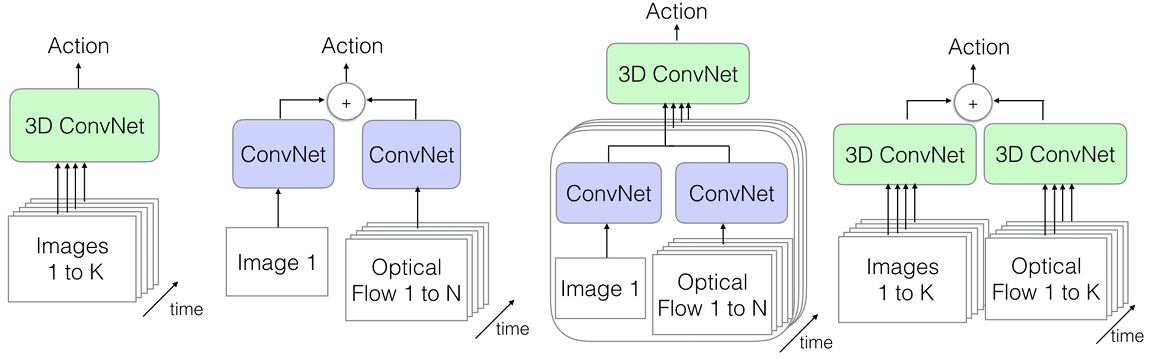
\includegraphics[width=.8\linewidth]{img/3DConvNet_approaches.JPG}
	\caption{Example from of previous RGB action recognition architectures, source from \cite{carreira2017quo}. (a) 3D-ConvNet. (b) Two-Stream. (c) 3D-Fused Two Stream. (d) Two-Stream 3D-ConvNet. K stands for the total number of frames in a video, whereas N stands for a subset of neighboring frames of the video.}\label{fig:3DConvNet}
\end{figure}


Moreover, several recent approaches have explored multi-modal fusion for enhanced action recognition. Methods combining RGB data with depth information or pose estimations have shown improved performance. For instance, \cite{franco2020multimodal}, \cite{tran2015learning} proposed a novel activity encoding method using temporal images from RGB video sequences and the integration of complementary information from a skeleton and temporal data. The proposed method outperforms state-of-the-art methods on public datasets. The challenges addressed in this paper include the difficulty of recognizing complex activities with high intra-class variability and the need for robustness to occlusions and noise. These challenges were addressed by using a multimodal approach that combines RGB and skeleton data, as well as a novel activity encoding method that uses temporal images. The limitations of this paper include the use of only two modalities (RGB and skeleton data) and the focus on recognizing activities in controlled environments. The proposed method may not generalize well to real-world scenarios with more complex backgrounds and lighting conditions.

RGB-based action recognition has witnessed remarkable progress, fueled by influential datasets and research papers. Despite these advancements, RGB-based action recognition still faces challenges. One major limitation is significant computational costs, making them less suitable for resource-constrained environments. However, ongoing research in the field aims to explore more efficient ways to handle large-scale labeled data and further improve the accuracy and robustness of RGB-based action recognition models.

With the advancements in pose estimation algorithms and models, annotating human pose estimation data with respective actions on a large scale has become more feasible. The availability of datasets containing 2D and 3D human skeleton information has significantly facilitated action recognition research. Human skeleton data provides a powerful representation that captures the essential structural and temporal information of actions while being resilient to environmental variations and occlusions. As a result, researchers have increasingly turned their attention to studying action recognition based on human skeletons. The benefits offered by skeleton-based action recognition methods, including improved robustness, reduced computational complexity, and better generalization across diverse scenarios, have led to a convergence of research efforts in this direction. In the next section, we will delve deeper into the advantages of using human skeleton representations for action recognition and explore the latest developments and methodologies in this rapidly evolving field.

\section{Action Recognition with Skeleton Data}
Action recognition with skeleton data is a crucial task in computer vision that involves identifying and categorizing human actions based on skeletal joint positions and temporal dynamics. Skeleton data is typically captured using depth sensors, motion capture systems, or pose estimation algorithms. Recent research has shown an increasing interest in skeleton-based action recognition due to its distinct advantages over other modalities, such as RGB data and depth sensors.

Skeleton data offers a compact and informative representation of human actions, focusing on the spatial arrangement and temporal dynamics of joints. Unlike RGB data, which requires complex processing to handle appearance changes and occlusions, skeleton data is inherently resilient to environmental variations, providing a robust representation for action recognition tasks. Additionally, compared to depth sensors, which can be sensitive to lighting conditions and limited in accuracy, skeleton data offers more precise and reliable joint information. One of the early skeleton action recognition datasets is the "NTU RGB+D" dataset introduced by \cite{shahroudy2016ntu}. This dataset contains 3D skeleton data captured by depth sensors, covering a diverse range of action classes and complex scenarios. Another notable dataset, the "Kinetics-Skeleton" dataset by \cite{kay2017kinetics}, provides 2D skeleton data extracted from videos in the Kinetics dataset, enabling a large-scale evaluation of skeleton-based action recognition models. Before the advent of deep learning, early methods of action recognition with skeleton data primarily relied on handcrafted features and traditional machine learning algorithms. These methods focused on extracting relevant information from the skeletal joint positions and designing effective classifiers to recognize actions. Major contributions during this era included the introduction of effective feature descriptors and the design of efficient classifiers.

One of the early approaches involved the use of histograms of joint angles or velocities as feature representations (e.g.,\cite{xia2012view}). By quantizing joint angles or velocities into bins and constructing histograms, these methods attempted to capture the spatial and temporal dynamics of actions. \cite{blank2005actions} is another approach involved the representation of actions as sequences of key poses or motion primitives. These key poses were identified based on keyframes or important points in the action sequences, providing a concise representation for recognition. Early methods also explored the application of traditional machine learning algorithms, such as Support Vector Machines (SVMs) and Hidden Markov Models (HMMs), to classify actions based on handcrafted features. These classifiers aimed to learn discriminative patterns from the extracted features and make predictions on new unseen sequences. However, these early methods had several limitations. Handcrafted feature engineering required domain expertise and manual design, making the process labor-intensive and potentially limiting the representation power of the features. Furthermore, these approaches struggled to successfully capture complicated spatio-temporal patterns, limiting their capacity to recognize actions with high accuracy. The lack of scalability and adaptability to large-scale datasets and diverse action scenarios posed challenges for real-world applications.

With the arrival of deep learning, there was a paradigm shift in skeleton-based action recognition, as an example shown in ~\ref{fig:skeletonPipeline}. Deep learning models, particularly recurrent and convolutional neural networks, revolutionized the field by automatically learning hierarchical and discriminative representations directly from skeleton data. These new approaches achieved remarkable performance improvements and demonstrated strong generalization capabilities across diverse action classes and scenarios. Recurrent Neural Networks (RNNs) enabled the modeling of temporal dependencies in action sequences, capturing the dynamics of actions over time. Convolutional Neural Networks (CNNs) were adapted to handle skeleton data by treating joint coordinates as image-like representations. Graph Convolutional Networks (GCNs) emerged to exploit the graph structure of skeleton data, effectively capturing spatial relationships between joints. Additionally, the introduction of attention mechanisms further enhanced the ability to focus on informative joints or temporal regions in the skeleton sequences. The integration of deep learning with skeleton-based action recognition has significantly improved accuracy, robustness, and scalability. These new approaches have sparked a surge of interest in the research community, leading to ongoing advancements and novel methodologies to explore the potential of deep learning in making use of the rich information present in skeleton data for action recognition tasks.

\begin{figure}
	\centering
	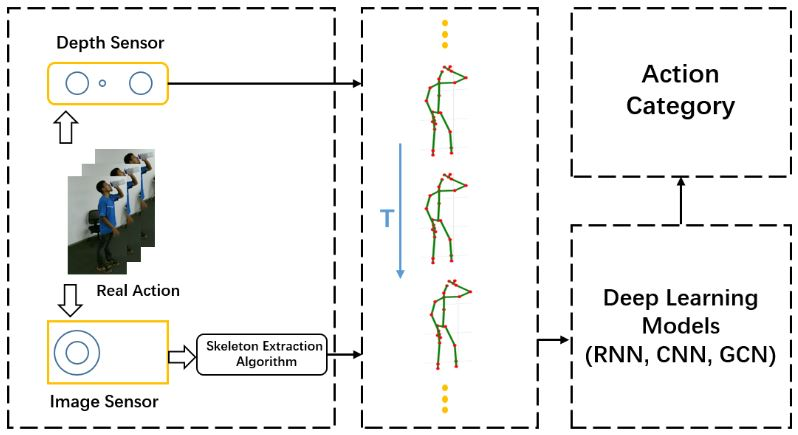
\includegraphics[width=.8\linewidth]{img/skeletonPipeline.JPG}
	\caption{Example from \cite{ren2020survey} the general pipeline of skeleton-based action recognition using deep learning methods. In the beginning, the skeleton data was gathered in two ways: directly from depth sensors or through pose estimate techniques.  The skeleton will be fed into neural networks based on RNN, CNN, or GCN.  Finally, we get to the action category.}\label{fig:skeletonPipeline}
\end{figure}

\subsection{RNN-Based Methods}
Recurrent Neural Networks as ~\ref{fig:LSTMSkeleton}, have been widely adopted to capture temporal dependencies in skeleton sequences. Specifically, in \cite{zhang2018adding} the result of the prior time step is used as the input for the current time step to create a recursive connection inside an RNN structure. A novel approach to adding attentiveness to RNN neurons. The proposed method is a simple yet effective way to adaptively weight the input elements of an RNN block at each time step. Moreover, the proposed method reduces computational overhead compared to existing attention mechanisms and is flexible in adapting to different types of RNNs, such as LSTM or GRU. The proposed method called EleAtt-RNN block addresses the challenges of modeling complex sequential information with fixed-weight RNNs and the limitation of existing attention mechanisms that require additional parameters and computational overhead. However, The performance of various related methods (e.g., \cite{wu2014leveraging}, \cite{zhao2017two}) often was unable to achieve a competitive outcome due to the RNN-based architecture's poor spatial modeling capability.

\begin{figure}
	\centering
	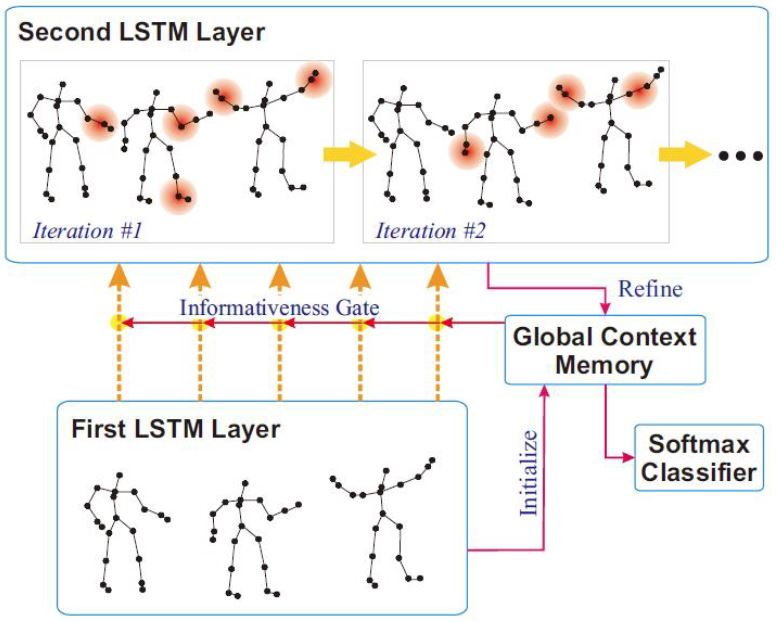
\includegraphics[width=.6\linewidth]{img/LSTMSkeleton.JPG}
	\caption{Example of RNN pipeline from \cite{Liu_2018} demonstrates how each joint has a distinct level of necessity for a specific skeleton action.}\label{fig:LSTMSkeleton}
\end{figure}
 
\subsection{CNN-Based Methods}
Convolutional Neural Networks have been extended to handle skeleton data by treating joint coordinates as image-like representations. Unlike RNNs, which explicitly model temporal dependencies in sequences, CNNs were originally designed for image-based tasks and lacked inherent temporal modeling capabilities. However, researchers have creatively adapted CNN architectures to effectively handle skeleton data by exploiting skeleton sequence data from vector sequence to pseudo-image. The main benefit of CNN-based methods over RNNs lies in their ability to efficiently capture spatial relationships among joints. CNNs are adept at learning hierarchical representations from image data, effectively recognizing local patterns and capturing spatial dependencies. This property aligns well with the inherent structural information in skeleton data, where each joint's position relies on its relationship with neighboring joints. This spatial awareness allows CNNs to learn discriminative features from skeleton sequences and recognize actions based on joint configurations and their temporal dynamics.\cite{ding2017investigation} investigate encoding richer spatial features into texture color images or 2D pseudo-images for 3D human action recognition using a CNN-based approach. Each type of feature is encoded into images in two or more ways to further explore the spatio-temporal information. The proposed method consists of five main components: spatial feature extraction from input skeleton sequences, key feature selection, texture color image encoding from key features, CNN model training based on images, and score fusion. One of the challenges that this paper solves is the limitation of using only joint positions for skeleton-based action recognition. By encoding richer spatial features into texture color images, the proposed method is able to capture more detailed information about the motion and shape of the human body, leading to improved recognition accuracy.

Still, this type of approach is a little complex and also misses out on crucial data throughout the mapping process. To address this problem, \cite{li2017skeleton} propose a translation-scale invariant transformation approach to map 3D skeleton videos to color images with enhanced temporal frequency adjustment capabilities, using a multi-scale deep CNN. Each frame's human skeleton joints were initially divided into five main sections in accordance with human physical structure, and those sections were then transferred to 2D form. With this technique, the skeleton picture is created using both spatial and temporal information. In addition, they employ various data augmentation methods specifically designed for 3D skeleton data to improve the generalization ability of the network. Still, even though the way it performed was enhanced, there is still no reason for treating the skeleton's joints as isolated entities since in the real world, our bodies are highly interconnected. For instance, when walking, other body parts like the hands and the hip should also be taken into consideration in addition to the joints directly within the legs. The shape-motion representation derived from geometric algebra was presented by \cite{li2019learning}, addressed the significance of both joints and bones, and completely utilized the data offered by the skeleton sequence, as shown in ~\ref{fig:3DCNN_shapeMotion}.

\begin{figure}
	\centering
	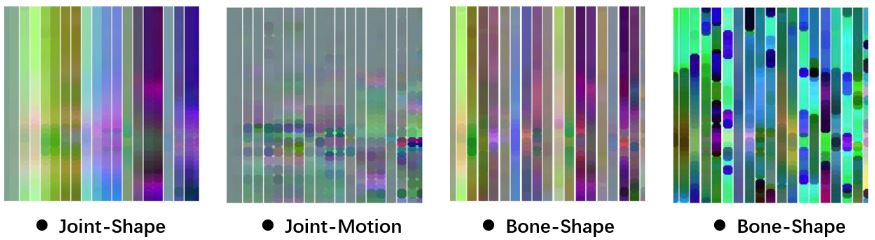
\includegraphics[width=.7\linewidth]{img/3DCNN_shapeMotion.JPG}
	\caption{Demonstration of the shape-motion representation given out by \cite{li2019learning}.}\label{fig:3DCNN_shapeMotion}
\end{figure}

 In this context, each skeleton joint is treated as a row and column in an image, and temporal dynamics are encoded through convolutional operations. However, this approach limits the consideration of co-occurrence features among all joints, as only neighboring joints within the convolutional kernel are considered. As a result, crucial correlations that may be related to the entire skeleton structure might be overlooked, preventing CNNs from learning comprehensive and useful features. Researchers have attempted to tackle this issue and enhance the representation capabilities of CNNs for skeleton data. \cite{li2018co} proposed an innovative end-to-end framework that employs a hierarchical approach to aggregate different levels of contextual information gradually. Firstly, point-level information is independently encoded, and then it is assembled into a semantic representation in both the temporal and spatial domains. By learning co-occurrence features with this approach, the model gains a more comprehensive understanding of the relationships among skeleton joints, improving its ability to recognize complex actions. Other challenges persist in these methods as the size and speed of the model, which can hinder real-time applications and require substantial computational resources. \cite{yang2019make} delves into techniques for optimizing CNN architectures to achieve more efficient models without sacrificing accuracy. Moreover, CNN-based methods can be sensitive to occlusions, viewpoint changes, and other variations in action sequences. Researchers have explored solutions to improve the robustness of CNNs in handling these challenges. For instance, \cite{liu2017enhanced} investigates methods to enhance skeleton visualization for improved action recognition under varying viewpoints.

 In summary, while CNN-based methods have shown promising results in skeleton action recognition, they face unique challenges related to co-occurrence feature learning, model efficiency, and robustness. Researchers continue to explore novel architectures, aggregation techniques, and optimization strategies to address these issues and advance the capabilities of CNNs in effectively recognizing actions from skeleton data. As an ongoing open problem, further investigation and innovation in CNN-based techniques hold the potential to unlock even more robust and accurate skeleton action recognition models.
 
\subsection{GCN-Based Methods}
The inherent topological graph structure of human 3D-skeleton data sets it apart from traditional sequence vectors or pseudo-images typically used in RNN-based or CNN-based methods. In recent years, Graph Convolutional Networks (GCNs) have emerged as a popular choice for effectively representing and processing graph-structured data, including skeleton graphs. There are two main types of graph-related neural networks: Graph and Recurrent Neural Networks (GNN) and Graph and Convolutional Neural Networks (GCN), research was focused primarily on the latter. The application of GCNs to skeleton-based action recognition has shown promising results, displaying convincing performance on various benchmarks. Unlike simply encoding skeleton sequences into sequence vectors or 2D grids, GCNs offer the ability to fully express dependencies between correlated joints. These networks, as a generalization of CNNs, can be applied to arbitrary structures, making them suitable for modeling the complex connectivity in skeleton graphs.

One notable model that utilizes GCNs for skeleton-based action recognition is the "Spatial Temporal Graph Convolutional Networks" (ST-GCN) presented in \cite{yan2018spatial}. This novel approach constructs a spatial-temporal graph with joints as graph vertices and natural connectivities in both human body structures and time as graph edges. The ST-GCN model learns higher-level feature maps on the graph and subsequently classifies them using a standard Softmax classifier to predict the corresponding action category. Since the introduction of ST-GCN, the use of GCNs for skeleton-based action recognition has garnered significant attention, leading to various related works. Researchers have focused on efficiently utilizing skeleton data and exploring richer dependencies among joints. For instance, "Actional-Structural Graph Convolutional Networks" (AS-GCN), proposed in \cite{li2019actional}, not only recognizes a person's action but also employs a multi-task learning strategy to predict the subject's next possible pose. The constructed graph in AS-GCN captures richer dependencies through two modules: Actional Links and Structural Links, as shown in ~\ref{fig:GCN_method}.

However, the most common concern across GCN-based action recognition studies remains data-driven, aiming to uncover the latent information hidden within 3D skeleton sequence data. The challenge lies in acquiring and transforming the skeleton data into a graph representation while preserving its temporal-spatial coupling and considering the connections among joints and bones. Another significant concern and challenge in GCN-based action recognition lies in effectively handling temporal dependencies within skeleton sequences. While GCNs are adept at capturing spatial relationships among joints in a single frame, they may struggle to explicitly model long-range temporal dependencies that span multiple frames. This limitation can impact the model's ability to recognize complex actions that involve intricate temporal dynamics.

\begin{figure}
	\centering
	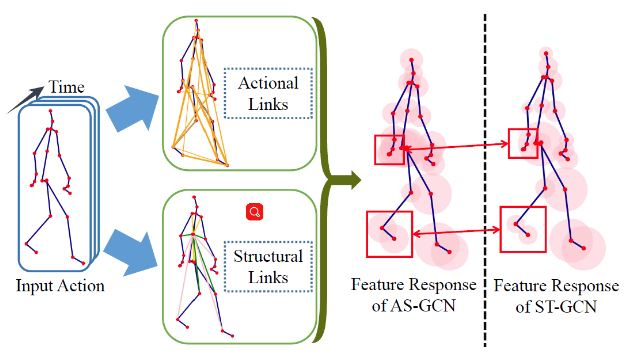
\includegraphics[width=.7\linewidth]{img/GCN_method.JPG}
	\caption{Demonstration of the feature learning in AS-GCN \cite{li2019actional} with generalized skeleton graphs. The actional links and structural links capture dependencies between joints. Compared to ST-GCN, AS-GCN obtains responses on collaborative moving joints (redboxes).}\label{fig:GCN_method}
\end{figure}


\subsection{Self-Attention Mechanism-Based Methods}
The revolutionary Transformer model, as introduced in \cite{vaswani2017attention} has made significant strides in natural language processing and has since been adopted in various domains, including computer vision. At the core of the Transformer's success lies its self-attention mechanism, which allows it to learn relationships between elements within a sequence effectively. This key feature enables Transformers to handle long sequences, a limitation that GCNs face as we mentioned before, and also traditional LSTM and RNN networks struggle with. The multi-headed self-attention mechanism further boosts efficiency by processing sequences in parallel, departing from the recursive word-by-word approach of LSTM and RNN networks. The advantages of self-attention have paved the way for its application in computer vision tasks, such as image classification and recognition, as demonstrated in \cite{wu2021cvt}. This work combines the strengths of CNNs and self-attention to model both local and global dependencies in images, resulting in improved performance for image classification tasks. Similarly, in \cite{bertasius2021space} self-attention was applied to learn spatio-temporal features from sequences of frame-level patches for video action recognition. The method effectively captured both spatial and temporal relationships, enhancing the model's ability to understand complex actions in videos.

Inspired by the success of Transformers and self-attention in computer vision, researchers have extended these principles to skeleton action recognition. In \cite{plizzari2021skeleton} the authors introduced a novel approach that utilizes self-attention instead of regular graph convolutions in both spatial and temporal dimensions. This extension of self-attention into the graph structure of skeleton data allowed the model to effectively capture dependencies between joints in space and time, leading to improved action recognition performance. By incorporating self-attention into the GCN framework, this method enables more comprehensive modeling of the complex interactions among skeleton joints, addressing the challenge of effectively capturing long-range temporal dependencies. Since distinct body components (such the arms and legs in "walking") between adjacent frames move simultaneously, the correlation of different joints across frames, which the previous Transformer-based approaches cannot capture, is particularly useful. The STTFormer is an approach in \cite{qiu2022spatio}, which is a novel spatio-temporal tuples transformer, where the skeleton sequence is broken up into multiple sections, and each portion has numerous consecutive frames that are encoded. The link between various joints' non-consecutive frames is then captured by a spatio-temporal tuples self-attention module (STTA). In order to improve the capacity to differentiate identical activities, a feature aggregation module (IFFA) was also included between non-adjacent frames. This model has shown better performance on benchmark datasets when compared to state-of-the-art methods. In this study, we will use ST-GCN, and the self-attention mechanism with the STTFormer model to investigate the capabilities of both techniques on different frameworks and learning strategies such as self-supervised learning which will discuss in the following section.

\section{Self-Supervised Learning}
Traditional supervised learning methods for computer vision tasks require large annotated datasets, which can be time-consuming and expensive to produce. Additionally, unsupervised learning methods lack guidance and may not generate meaningful representations. Self-Supervised Learning (SSL) offers a compelling solution to these challenges by leveraging unlabeled data to learn useful representations without the need for external annotations. Self-Supervised Learning is a branch of machine learning where a model learns to predict or reconstruct certain parts of its input data without explicit supervision. The model is trained to solve pretext tasks, which are constructed from the data itself, rather than relying on externally labeled datasets.

By employing pretext tasks, the model learns to capture meaningful features from the data, which can then be transferred to downstream tasks, as shown in ~\ref{fig:SSL_pipeline}. In supervised learning, the model is trained on labeled data with input-output pairs, whereas in unsupervised learning, the model aims to discover underlying patterns in unlabeled data. SSL falls between these two paradigms, utilizing unlabeled data and transforming it into labeled-like data by creating pretext tasks that serve as supervisory signals for training.



\subsection{SSL: Pretext Tasks}
Early research in SSL explored various pretext tasks to effectively exploit unlabeled data. A common approach involved training models to predict missing parts of an input image, such as inpainting or image completion tasks. By predicting masked-out regions, the model learned to understand contextual relationships within the image. Papers such as \cite{pathak2016context} and \cite{yu2018generative} delved into this area. In \cite{gidaris2018unsupervised} contributed to the development of another prevalent pretext task was image rotation, where the model learned to predict the rotation angle applied to an image. This task encouraged the model to capture semantic information and invariant features in different orientations. Recent advancements in SSL have explored novel approaches, including pretext tasks and contrastive learning methods. One notable research direction focuses on pretext tasks, where the model learns from multiple transformations of the same input data, such as jigsaw puzzles in \cite{noroozi2016unsupervised}, colorization \cite{larsson2016learning}. These pretext tasks offer diverse learning signals, leading to more robust feature representations. is a pioneering work in this area.

\begin{figure}
	\centering
	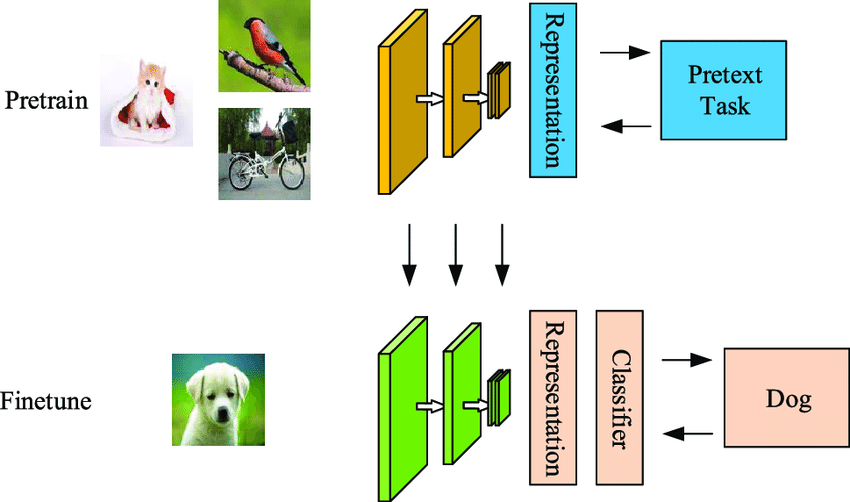
\includegraphics[width=.7\linewidth]{img/SSL_pipeline.png}
	\caption{The general pipeline for SSL from pre-training the model with a pretext task then transferring to a downstream task, source from \cite{v7labs2022ssl}.}\label{fig:SSL_pipeline}
\end{figure}


\subsection{SSL: Contrastive Learning}
On the other hand, contrastive learning has gained popularity, where the model is trained to pull similar instances closer in the embedding space while pushing dissimilar instances apart, as shown in ~\ref{fig:ContrastiveLearning}. This method enables the model to learn high-level feature representations that effectively capture the inherent structure of the data. One of the pioneering works in contrastive learning is (CPC) \cite{oord2018representation}. CPC formulates a pretext task where the model predicts future audio segments given past segments. The key insight behind CPC is to contrast the predictions of true future segments with other negative samples, forcing the model to learn representations that capture relevant information for future prediction. Papers such as \cite{he2020momentum} and \cite{chen2020simple} have significantly contributed to the advancements in contrastive learning. \cite{he2020momentum} leveraged momentum contrast to create a contrastive loss. The model uses a moving average of the model's weights, known as the momentum encoder, to generate a key representation for each data sample. The main encoder then generates a query representation, and the contrastive loss encourages the model to maximize agreement between the query and key representations for positive samples while minimizing agreement for negative samples.

One of the primary challenges in early contrastive learning methods was the choice of negative samples. In the CPC method, selecting negative samples from the same audio sequence resulted in the model learning trivial solutions. To overcome this, researchers introduced more sophisticated strategies to create informative negative samples, such as using samples from other data instances or different time steps. Additionally, contrastive learning was computationally demanding as it required comparing each positive sample with all possible negative samples. Early research explored techniques to speed up the process, such as using large memory banks for negative samples and employing batch normalization for efficiency.

Recent research as \cite{chen2020simple} introduced the SimCLR framework, which demonstrated the effectiveness of large-batch contrastive learning and data augmentation plays a critical role in defining effective predictive tasks. However, a limitation of SimCLR lies in its reliance on large batch sizes, which might not be practical for all hardware configurations. Another notable work is (SwAV) \cite{caron2020unsupervised}, which proposed a novel clustering-based approach for contrastive learning. While SwAV achieved impressive results, its success relies on having a large number of data samples, which might pose challenges for small-scale datasets.

In \cite{grill2020bootstrap}, the authors introduced (BYOL) an innovative approach to self-supervised learning that are negative-sample-free and not relying on negative pairs, which solves the issue of mining the relevant negative pairs and it doesn't need the explicit generation of negative sample pairs. In \cite{caron2021emerging} (DINO) they were inspired by (BYOL) and they proposed an asymmetric network based only on positive pairs to prevent feature collapse. This recent research achieved state-of-the-art results by leveraging an ensemble of neural networks to learn and bootstrap their own unsupervised representations.

\begin{figure}
	\centering
	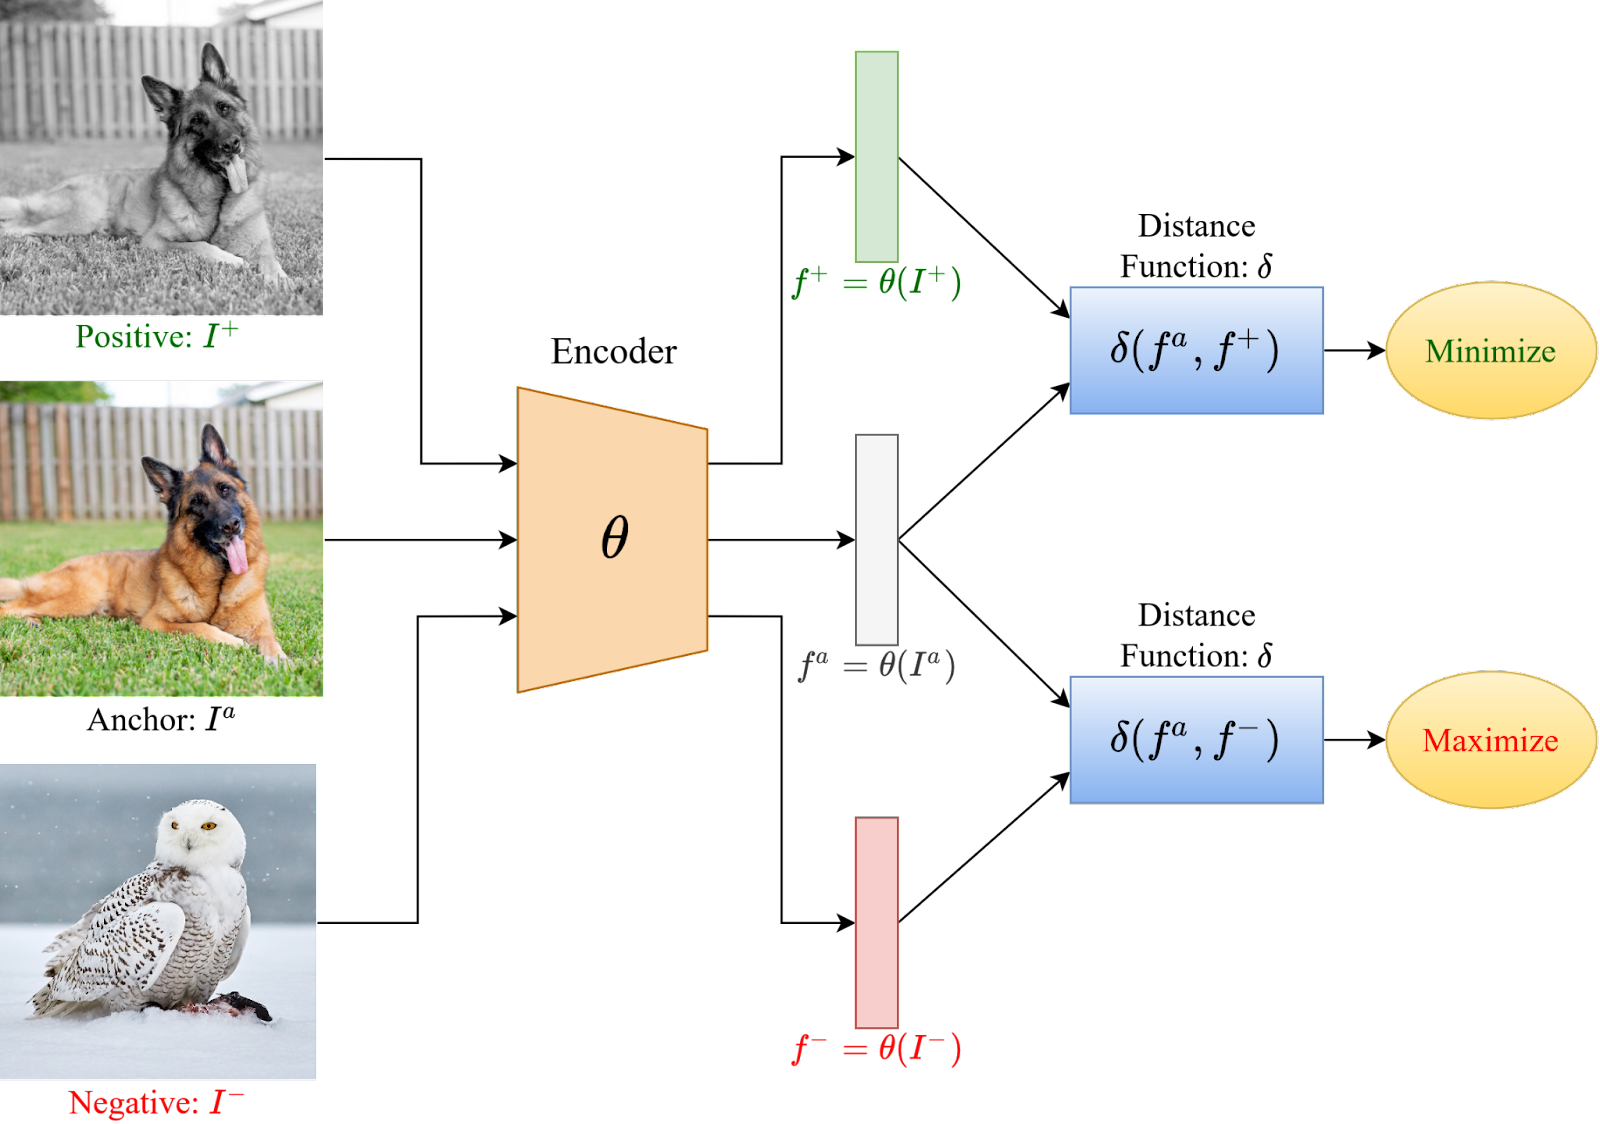
\includegraphics[width=.6\linewidth]{img/ContrastiveLearning.png}
	\caption{Demonstration in \cite{v7labs2022contrastive} of contrastive learning by minimizing the similarity function between the anchor and the positive sample, and maximizing the distance between the anchor and the negative sample.}\label{fig:ContrastiveLearning}
\end{figure}


\subsection{Evaluating SSL models}

Evaluating the performance of SSL methods requires careful consideration due to the absence of traditional supervised labels. Researchers have devised various evaluation techniques to assess the quality of learned representations and the effectiveness of pretext tasks in capturing meaningful features.

One common evaluation metric in SSL is the "linear evaluation protocol," where the learned representations are fine-tuned on downstream tasks using simple linear classifiers. By using linear classifiers, researchers can measure the quality of the learned features without introducing additional complexity from complex classifiers or fine-tuning the entire model. The performance of these linear classifiers on downstream tasks serves as a proxy for evaluating the generalization capability of the learned representations. Another crucial aspect of SSL evaluation involves assessing how well the learned representations transfer to downstream tasks. SSL models aim to capture high-level features, which should be transferable to various computer vision tasks. Transfer learning to tasks such as image classification, object detection, and semantic segmentation can be employed to evaluate the effectiveness of learned representations in real-world applications.

A key evaluation consideration in SSL is the comparison between fine-tuning the entire model and using a linear classifier on top of the frozen backbone. Fine-tuning the entire model on downstream tasks allows for further adaptation to specific task domains, potentially achieving higher task-specific performance. However, fine-tuning may lead to overfitting or require a substantial amount of labeled data, which defeats the purpose of SSL. On the other hand, using linear classifiers on top of the frozen SSL backbone is computationally efficient and avoids overfitting issues. This approach allows researchers to evaluate the transferability of learned representations without requiring additional labeled data for fine-tuning. Although fine-tuning may yield better results on task-specific metrics, linear evaluation provides valuable insights into the generalization capabilities of the SSL model across different tasks.

The success of SSL lies in its ability to learn generic feature representations, which can be transferred to a wide range of downstream computer vision tasks. Some common downstream tasks include:

\begin{itemize}
	\item \textbf{Classification:} Evaluating the SSL model's ability to classify objects on the learned features. This is one of the most common and widely used downstream tasks for SSL evaluation.

	\item \textbf{Object Detection:} Assessing the performance of the SSL model on detecting and localizing objects within an image. This task evaluates the representations' capacity to capture object-level information.

 	\item \textbf{Semantic Segmentation:} Evaluating the model's ability to segment an image into different object categories or regions. This task tests the model's capability to understand spatial relationships within an image.

  	\item \textbf{Action Recognition:} Assessing the model's performance on recognizing and classifying actions from video sequences. This task examines the representation's ability to capture temporal dynamics.

   	\item \textbf{Domain Adaptation:} Evaluating the transferability of learned representations across different domains or datasets. This task is critical for assessing SSL models' generalization across various real-world scenarios.
     
\end{itemize}

In conclusion, Self-Supervised Learning presents a compelling alternative to traditional supervised and unsupervised learning approaches, harnessing the potential of unlabeled data to learn informative representations. Through pretext tasks and contrastive learning, SSL has demonstrated remarkable success in solving computer vision tasks and continues to be an active area of research in the field of machine learning.



\section{Self-supervised skeleton-based action recognition}
Self-supervised learning has emerged as a promising approach for learning informative representations from unlabeled data in the context of skeleton-based action recognition. Researchers have explored various self-supervised techniques to leverage the temporal dynamics and spatial information present in skeleton data. In the paper \cite{zheng2018unsupervised} the authors proposed a method based on a recurrent encoder-decoder GAN to reconstruct the input skeleton sequence. By learning to reconstruct the input sequence, the model can capture long-term temporal dynamics and subtle motion patterns essential for action recognition. Building on the ideas of reconstruction, the research (Predict\&Cluster) in \cite{su2020predict} introduced a decoder to improve the representation ability of the encoder. The method leverages both prediction and clustering to encourage the model to learn more discriminative and compact representations.

In \cite{lin2020ms2l} authors proposed (MS2L) a multi-task framework, including motion prediction and jigsaw puzzle tasks, to enhance the model's understanding of motion and spatial relationships among joints. By jointly solving multiple tasks, the model can capture richer information from the skeleton sequences. (AS-CAL) was introduced in \cite{rao2021augmented} as an approach that utilizes momentum LSTM to regularize the feature space. Along with various skeleton augmentation strategies, this method aims to enhance the model's robustness and generalization capability. In \cite{li20213d} proposed SkeletonCLR, which applies a memory bank to store negative samples and employs a cross-view knowledge mining strategy. By leveraging the memory bank and cross-view consistency, the model can capture more comprehensive and discriminative representations. In order to add movement patterns and compel the encoder to acquire broader representations, (AimCLR)  proposes to make extensive use of augmentation.  The amount of redundant information within the spatial joints and temporal frames, which might increase the strength of 3D visual representation and are crucial for downstream tasks, has not been taken into account. These contrastive learning approaches, on the other hand, significantly rely on powerful data augmentation procedures.

The Partial Spatio-Temporal Learning (PSTL) is a recent research published in 2023 in \cite{zhou2023self} proposed to address the limitations of existing methods in skeleton-based action recognition. While current approaches focus on a global perspective to discriminate different skeletons, PSTL aims to leverage the local relationship between various skeleton joints and video frames, which is crucial for real-world applications. PSTL adopts a unique spatio-temporal masking strategy to construct partial skeleton sequences, allowing the model to focus on specific regions of interest. The framework utilizes a negative-sample-free triplet stream structure, comprising an anchor stream without any masking, a spatial masking stream with Central Spatial Masking (CSM), and a temporal masking stream with Motion Attention Temporal Masking (MATM). These innovative components facilitate the exploitation of local dependencies and cues within the skeleton sequences, ultimately leading to improved action recognition performance. As part of this research, we will further investigate the efficacy of PSTL with different settings and diverse datasets to comprehensively validate its potential in advancing skeleton-based action recognition.
\chapter{Methodology}
In this section, we present the methodology for self-supervised skeleton-based action recognition, exploring two distinct approaches to leverage the benefits of self-supervised learning: DINO with STTFormer and PSTL with ST-GCN. We will compare their performance on benchmark datasets, highlighting learning strategies, and data preprocessing. First we propose an approach inspired by the DINO framework introduced in \cite{caron2021emerging}. Unlike the original DINO, which focuses on image data, our adaptation is designed explicitly for 3D skeleton data. In the DINO framework, the self-distillation technique is applied, wherein a vision transformer is used as the teacher network. In our context, we leverage the momentum encoder of STTFormer as the teacher network, predicting its output directly. We use a standard cross-entropy loss to align the student and teacher predictions, effectively learning meaningful representations without the need for labeled data. The core idea is to utilize the STTFormer, a spatio-temporal transformer-based network, as the encoder for our self-supervised learning. The second approach we explore is the Partial Spatio-Temporal Learning (PSTL) framework, a method explicitly designed for skeleton-based action recognition. In this approach, we employ the ST-GCN architecture as the backbone.

For our experiments, we will employ the existing PSTL framework and compare it with the DINO approach. The first approach utilizes the combination of PSTL with ST-GCN as the encoder. Our second approach, which is our contribution, employs a new combination of DINO and STTFormer as an encoder. For both approaches, we adopt self-supervised learning strategies, where the model learns to make meaningful predictions from the unlabeled skeleton data. This allows us to overcome the limitations of traditional supervised methods, which rely on costly and time-consuming data annotation. During training, we employ data preprocessing techniques to prepare the skeleton data for learning. This includes normalization, joint alignment, and temporal synchronization. Additionally, we apply data augmentation to increase the diversity of the training set and enhance the robustness of the learned representations. The goal is to identify the strengths and weaknesses of each method, providing valuable insights into the application of self-supervised learning for skeleton-based action recognition.

\section{First Approach Overview: DINO \& STTFormer}
The success of the DINO framework in self-supervised learning for images, where a transformer serves as the backbone, has motivated us to explore its potential for skeleton-based action recognition. Transformers have demonstrated remarkable capabilities in learning meaningful representations from data, especially in self-supervised learning tasks. Leveraging the success of transformers in SSL, we propose to use the STTFormer as the backbone in our DINO-inspired approach. In our DINO-inspired approach, we employ two streams with the same encoder, the STTFormer. As shown in ~\ref{fig:DINO_pipeline}The architecture consists of an upper stream, representing the student, and a lower stream, acting as the teacher. The primary objective is for the student to learn good representations from the teacher. The key feature is the self-distillation technique, where the teacher network guides the learning of a student network through cross-entropy loss. 
The student learns from the gradients backpropagated through the loss function during training. However, there is a stop gradient applied to the teacher to prevent direct influence from the student's updates. Instead, the teacher learns from the exponential moving average of the student's weights, creating a smoother and more stable learning process.

The encoder in our approach utilizes spatio-temporal tuples encoding to capture both spatial and temporal relationships within the skeleton data. This encoding strategy allows the model to extract meaningful joint interactions and motion patterns essential for accurate action recognition.

\begin{figure}
	\centering
	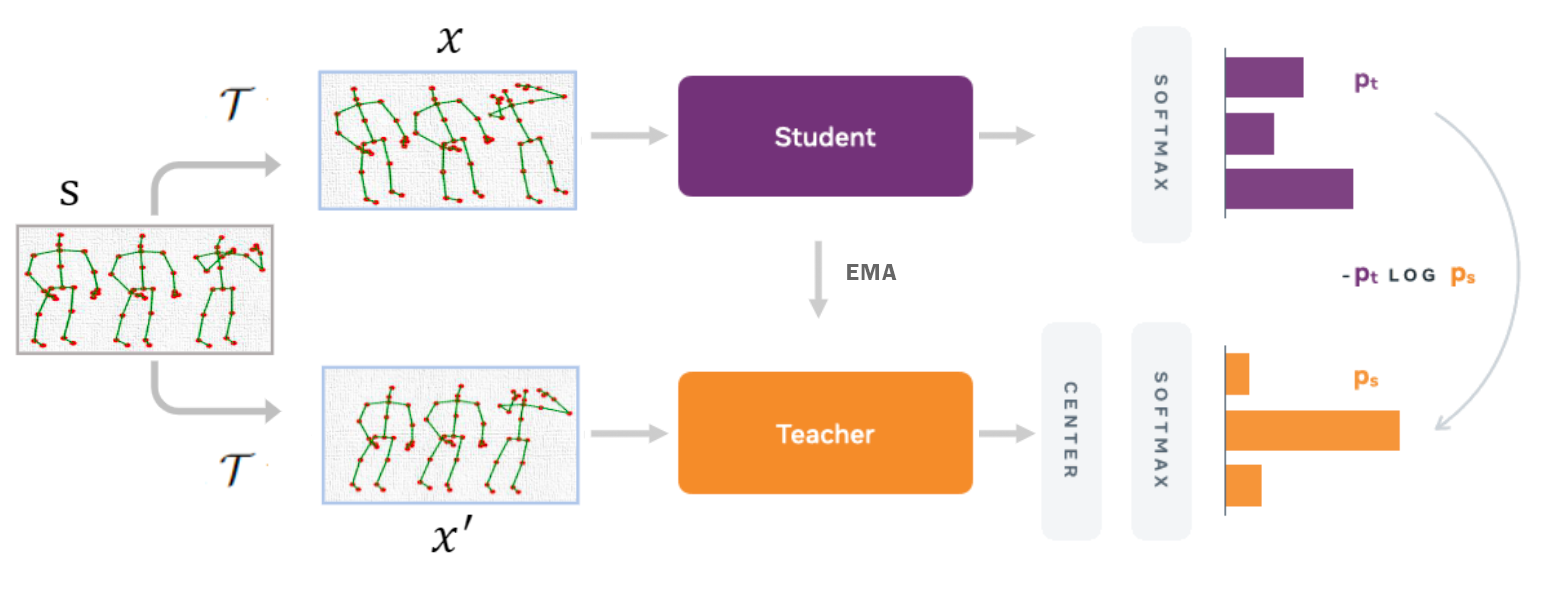
\includegraphics[width=.9\linewidth]{img/DINO_pipeline.png}
	\caption{Illustration of the DINO framework where The model passes two different random transformations (x,x') of an input image s to the student and teacher networks.}\label{fig:DINO_pipeline}
\end{figure}

In the following section, we provide a comprehensive breakdown of each component within the Spatio-Temporal Tuples Transformer. This includes detailed descriptions of self-attention mechanisms with (STTA) blocks, and Inter-Frame Feature Aggregation (IFFA). We also elaborate on positional encoding and its significance in capturing the sequential dependencies of skeleton data.

\subsection{Backbone Encoder: STTFormer}
Spatio-Temporal Tuples Transformer (STTFormer) is a novel method for skeleton-based action recognition that captures the dependencies between joints and achieves better performance on large-scale datasets. The overall architecture of STTFormer is shown in ~\ref{fig:STTFormer}. The input is a skeleton sequence with $V_0$ joints and $T_0$ frames. The sequence is divided into $T$ parts, each containing $n$ consecutive frames, for a total of $V = n * V_0$ joints. Then, a tuple encoding layer is utilized to encode each tuple data. A total of $L$ layers are stacked in the spatio-temporal tuples Transformer, and each layer is composed of Spatio-Temporal Tuples Attention (STTA) and Inter-Frame Feature Aggregation (IFFA). Finally, the obtained features are input into a global average pooling layer and a fully connected layer to obtain classification scores.

\begin{figure}
	\centering
	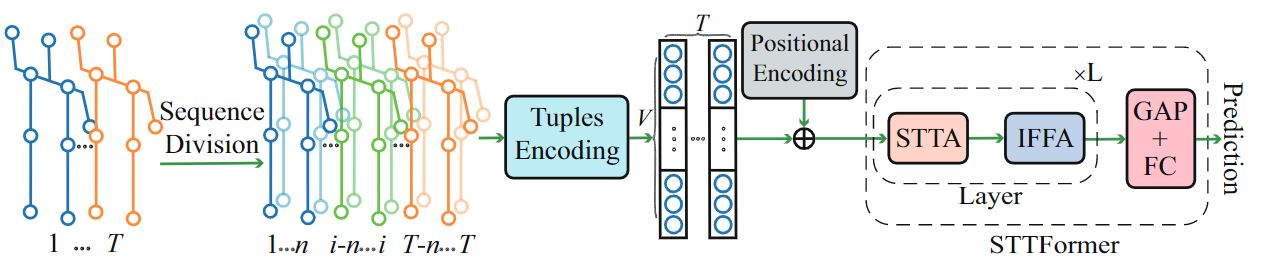
\includegraphics[width=.9\linewidth]{img/STTFormer.JPG}
	\caption{Illustration from \cite{qiu2022spatio} shows the overall architecture of the STTFormer. It consists of two main blocks: the spatio-temporal tuples encoding and  spatio-temporal tuple Transformer.}\label{fig:STTFormer}
\end{figure}


At the beginning of the Spatio-Temporal Tuples Encoding phase, each tuple is flattened into a short sequence, as the raw skeleton sequence
\(X_0 \in \mathbb{R} ^{ C_0 \times T_0 \times V_0}\) is fed to a feature mapping layer to expand the input channel to a set number $C_1$. Subsequently, the skeleton sequence is divided into $T$ non-overlapping tuples:

\begin{center}
$X = [x_1,x_2, ..., x_T], x_i \in \mathbb{R}^{C_1\times n \times V_0}$
\end{center}

Then the tuples sequence goes through a flattening layer:

\begin{center}
$X \in \mathbb{R}^{C_1 \times T \times n \times V_0} \to \mathbb{R}^{C_1 \times T \times V}$
\end{center}

where $T = T_0/n, V = n \times V_0$. Then a positional encoding strategy is used to encode the temporal and spatial information of each joint in the tuple. Specifically, each joint is represented by a vector of its 3D coordinates, and the temporal information is represented by a vector of its frame index. Then, the positional encoding is applied to each vector to capture the relative position of each joint in the tuple, as shown in ~\ref{fig:STTFormer_tuplesEncoding}. The positional encoding is defined as follows:

$$PE_{(pos,2i)} = sin(pos/10000^{2i/C_{in}})$$
$$PE_{(pos,2i+1)} = cos(pos/10000^{2i/C_{in}})$$

where $pos$ is the position of the joint in the tuple, $i$ is the index dimension of the position encoding vector, and $C_in$ is the dimension of the joint vector. The output of the encoding is defined as $X_{in}$

In the Spatio-Temporal Tuples Attention phase, a self-attention mechanism is used to capture the relationship between joints in each tuple. Specifically, a spatio-temporal tuple self-attention (STTA) module is used to extract the related features of joints in each short sequence. The STTA module is defined as follows, the encoded sequence $X_{in}$ is projected into the query $Q$, key $K$ and value $V$:


\begin{center}
$Q,K,V = Conv_{2D(1\times1)}(X_{in})$
\end{center}

Like the standard Transformer, the dot-product is used as the similarity function, the $Tanh$ function is utilized to normalize the obtained weights.

$$X_{attn}(Q,K,V) = Tanh(\frac{QK^T}{\sqrt{C}})V$$

Where $C$ denotes the number of channels of the key $K$, which can avoid excessive inner product to increase gradients stability during training. The output of the STTA module is a weighted sum of the value matrix $V$, where the weights are determined by the final attention.

\begin{figure}
	\centering
	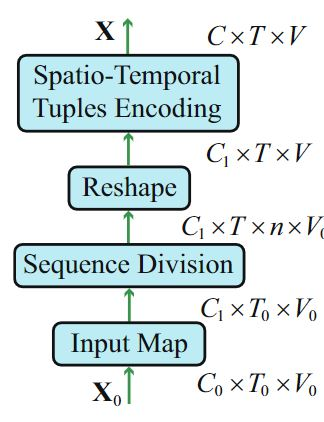
\includegraphics[width=.3\linewidth]{img/STTFormer_tuplesEncoding.JPG}
	\caption{Transformation of the input data through the spatio-temporal tuples encoding.}\label{fig:STTFormer_tuplesEncoding}
\end{figure}

To fuse the output, a feed-forward layer using $1\times1$ 2D convolution is added, resembling the transformer, as shown in ~\ref{fig:STTFormer_transoformer}.

A single action can be broken down into numerous smaller ones, such as the "long jump" which includes the "run-up," "take-off," and "landing" motions. Each tuple in the STTFormer contains a sub-action that was created by modeling a number of consecutive $n$ frames using STTA. The construction of a correlation between various sub-actions, such as "run-up," "take-off," and "landing," will aid in action recognition and aid in separating similar acts, such as high jump and long jump. In the Inter-Frame Feature Aggregation phase, a convolution operation with $k_2 \times 1$ kernel size is used to realize inter-frame feature aggregation in the temporal dimension. Specifically, the output of the STTA module is fed into a convolutional layer to aggregate the features of each joint across different frames. The IFFA operation is defined as follows:

$$X_{IFFA} = Conv_{2D(k_2 \times 1)}(X_{STTA})$$

where $X_{STTA}$ is the output of the STTA module, and $k_2$ is the kernel size. At last, the residual connections are used to stabilize network training as shown in ~\ref{fig:STTFormer_transoformer}. All outputs connected to the rest are regularized to prevent overfitting.


\begin{figure}
	\centering
	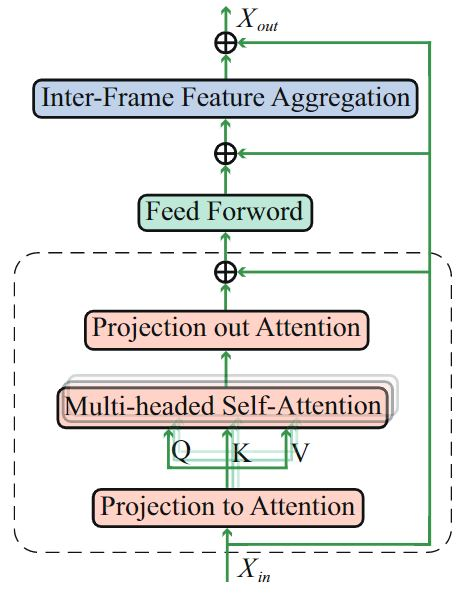
\includegraphics[width=.4\linewidth]{img/STTFormer_transoformer.JPG}
	\caption{An example of the suggested spatio-temporal tuples L of these layers make up the transformer layer, which is the whole STTFormer.}\label{fig:STTFormer_transoformer}
\end{figure}


\subsection{Learning Strategy: DINO}
In the DINO framework, the model processes two different random transformations of an input, in our method, we will pass two skeleton sequences. These transformations are passed through the student network, denoted as $g_{\theta_s}$, and the teacher network denoted as $g_{\theta_t}$. Both the student and teacher networks have identical architectures but differ in their parameters. The output of the teacher network is centered with a mean computed over the batch, resulting in a more stable and robust representation. Each network, i.e., the student and the teacher, produces a K-dimensional feature representation, denoted as $P_s$ and $P_t$, respectively, as shown in ~\ref{fig:DINO_pipeline}. These feature representations are then normalized using a softmax operation with a temperature $\tau_s$ over the feature dimension. This normalization step ensures that the features remain in a suitable range for learning and generalization:

\begin{center}
$P_s(x)^{(i)}=\frac{\exp \left(g_{\theta_s}(x)^{(i)} / \tau_s\right)}{\sum_{k=1}^K \exp \left(g_{\theta_s}(x)^{(k)} / \tau_s\right)}$,
\end{center}

The core of the DINO framework lies in the self-distillation process. With a fixed teacher, the similarity between the student and teacher features is measured using a cross-entropy loss:

\begin{center}
$\min _{\theta_s} H\left(P_t(x), P_s(x)\right)$
\end{center}

where:

\begin{center}
$H(a, b)=-a \log b$
\end{center}

More precisely, from a given skeleton sequence, a set $V$ of different skeleton augmentations is generated. This set contains two weak augmentations, $x^g_1$ and $x^g_2$ and several strong augmentations. All augmentations are passed through the student while only the weak augmentations are passed through the teacher, therefore we mimic the strategy of encouraging “local-to-global” correspondences used in images from the DINO paper. The loss then is minimized as:

$$
\min _{\theta_s} \sum_{x \in\left\{x_1^g, x_2^g\right\}} \sum_{\substack{x^{\prime} \in V \\ x^{\prime} \neq x}} H\left(P_t(x), P_s\left(x^{\prime}\right)\right)
$$

This loss function drives the student to learn meaningful and discriminative representations by mimicking the knowledge present in the teacher's feature space. A crucial aspect of DINO is the use of exponential moving average to update the teacher network's weights. The teacher network learns from the moving average of the student network's parameters, resulting in smoother and more consistent updates. This technique stabilizes the learning process and helps the student converge to better representations. 

The neural network $g$ is composed of a backbone $f$ which is the STTFormer, and a projection head $h$: $g=h\circ f$. The features used in downstream tasks are the backbone $f$ outputs. The projection head comprises of two layers of a multi-layer perceptron (MLP) with a hidden dimension of 512, l2 normalization, and a fully connected layer (Weight Norm) with weight normalization and K dimensions, as shown in ~\ref{fig:dino_illustrationv2}.

Centering and sharpening are used so that the first prevents one dimension from dominating while encouraging collapse to a uniform distribution, whereas sharpening does the reverse. The use of both processes balances the impact they have. Output sharpening is carried out by setting the temperature $\tau_t$ to a low value in the teacher's softmax normalization. This mechanism has been proven to make a similar impact as the negative samples in which it makes the system learn meaningful representations and prevent collapse to a uniform distribution, which makes the system negative-sample-free. 

\begin{figure}
	\centering
	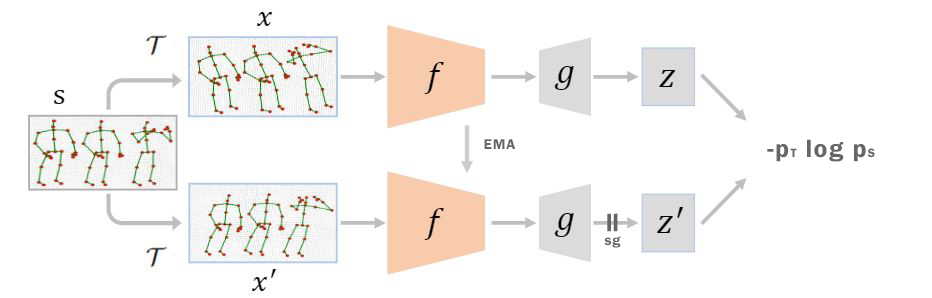
\includegraphics[width=.9\linewidth]{img/dino_illustrationv2.png}
	\caption{The output $h$ of the encoder $f$ go through a projection head $g$ to get embeddings $z$ and $z'$ for the student and the teacher, respectively .}\label{fig:dino_illustrationv2}
\end{figure}


\section{Second Approach Overview: PSTL \& ST-GCN}
The second approach in this study involves combining the "Partial Spatio-Temporal Learning" (PSTL) framework with the "Spatial Temporal Graph Convolutional Networks" (ST-GCN) as a backbone. This approach is motivated by the limitations of current contrastive learning-based methods in effectively leveraging the rich action clues stored in skeleton sequences. Current contrastive learning-based methods focus on finding effective global data augmentations to create various views of the skeleton. However, this global perspective may limit the model's ability to fully exploit the local relationships between different skeleton joints and video frames, especially in real-world scenarios. Moreover, these methods often require a large batch size or memory bank, making them unsuitable for scenarios with limited skeleton data. PSTL draws inspiration from the "Skeleton Barlow Twins" (SkeletonBT) method \cite{zbontar2021barlow}, which is known for its effective utilization of local relationships in skeleton sequences. Building on this idea, PSTL adopts a triple stream architecture, as shown in ~\ref{fig:pstl_pipline}. It applies Central Spatial Masking (CSM) on the spatial masking stream and Motion Attention Temporal Masking (MATM) on the temporal masking stream. Additionally, an extra anchor stream is included to retain the original semantic information.

\begin{figure}
	\centering
	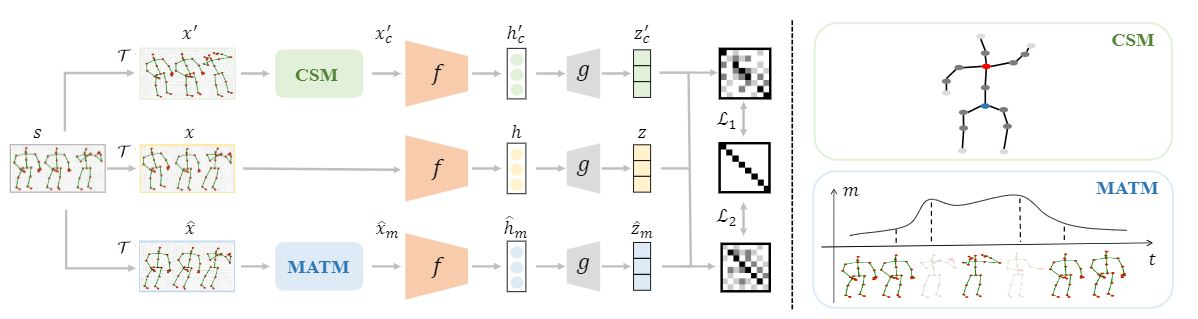
\includegraphics[width=.9\linewidth]{img/pstl_pipeline.JPG}
	\caption{ The general structure of PSTL representation in \cite{zhou2023self}.  Red, blue, dark gray, and light gray are the degrees for Central Spatial Masking (CSM). Motion Attention Temporal Mask (MATM) uses m to represent motion density and t to represent time.}\label{fig:pstl_pipline}
\end{figure}


Graph Convolution Networks (GCN) have demonstrated considerable success in the field of human action recognition. GCNs excel at processing data with graph structures, making them a suitable choice for handling skeleton-based action recognition tasks. The Spatial Temporal Graph Convolutional Networks (ST-GCN) model serves as the backbone for the PSTL framework. ST-GCN is capable of capturing both spatial and temporal dependencies within the skeleton sequences, and moreover, its stable results on different datasets make it well-suited for our study. The PSTL approach adopts a triple stream architecture, with all three streams utilizing the same encoder, which is the ST-GCN model. In the following section, each component of the ST-GCN model is described in detail. This includes a comprehensive explanation of how ST-GCN captures spatial and temporal information, processes graph structures, and extracts relevant features from skeleton sequences. By integrating the PSTL framework with the ST-GCN backbone, the second approach aims to overcome the limitations of current contrastive learning-based methods and enhance the model's performance and robustness in skeleton-based action recognition tasks. 

\subsection{Backbone Encoder: ST-GCN}
The Spatial Temporal Graph Convolutional Networks (ST-GCN) is a powerful model designed for action recognition tasks, specifically tailored for skeleton-based data. The motivation behind using graph convolution networks arises from the fact that skeletons are inherently represented in the form of graphs, where each node corresponds to a joint of the human body. This graph representation makes it challenging to utilize traditional models like convolutional networks, which are designed for 2D or 3D grids. The ST-GCN model is formulated on top of a sequence of skeleton graphs, where each graph represents a single frame of the action sequence. The graph nodes represent the joints of the human body, while the edges can be of two types: spatial edges that encode the natural connectivity of joints within the human body structure, and temporal edges that connect the same joints across consecutive timesteps in the action sequence, as shown in ~\ref{fig:STGCN_Illustration}. The core of the ST-GCN model lies in the construction of multiple layers of spatial temporal graph convolution. These layers enable the integration of information along both the spatial and temporal dimensions of the skeleton data. This integration allows the model to capture the spatial relationships between joints in a single frame as well as the temporal dependencies between corresponding joints across consecutive frames in the action sequence.

\begin{figure}
	\centering
	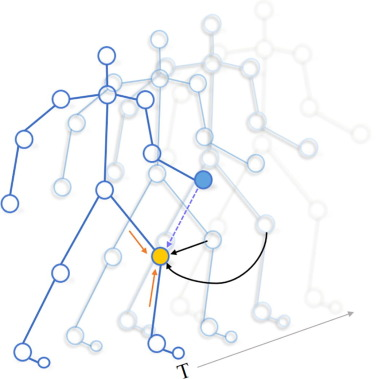
\includegraphics[width=.4\linewidth]{img/STGCN_Illustration.jpg}
	\caption{Illustration in \cite{peng2021rethinking} of modeling skeleton with ST-GCNs.}\label{fig:STGCN_Illustration}
\end{figure}

In ST-GCN, the graph denoted as $G = (V, E)$ is formed on a skeleton sequence with $N$ joints and $T$ frames, capturing both intra-body and inter-frame connections. The node set $V = \{v_{ti} \| t = 1,...,T,i=1,...,N\}$ includes all the joints in the skeleton sequence. The input to the ST-GCN model is represented by the feature vector on each node $F(v_{ti})$, which comprises the coordinate vectors and estimation confidence of the $i$-th joint on frame $t$. To construct the spatial temporal graph, the model perform the process in two steps:

\textbf{Intra-Skeleton Connection (Spatial Edges):} Within each frame, the joints are connected based on the natural connectivity of the human body structure. These connections, denoted as $E_S = \{v_{ti} v_{tj} \| (i,j) \in H\}$, are established using the set $H$, which specifies the naturally connected human body joints. This automatic assignment of connections ensures that the network architecture can handle datasets with varying numbers of joints or joint connectivities.

\textbf{Inter-Frame Connection (Temporal Edges):} Each joint is connected to the corresponding joint in the consecutive frame, forming inter-frame edges denoted as $E_F =\{v_{ti} v_{(t+1)i}\}$.
These inter-frame edges capture the temporal relationships and represent the trajectories of each joint over time. Thus, for a given joint $i$, all edges in $E_F$ will indicate its trajectory through time.

Spatial Graph Convolution allows the model to perform convolutional operations on the spatial graph, treating each frame independently and encoding the relationships between joints within a single frame. Let's delve into the details of the Spatial Graph Convolution. In this case, on a single frame at time $\tau$, we have $N$ joint nodes $V_t$, and the skeleton edges $E_S = \{v_{ti} v_{tj} \| t = \tau, (i,j) \in H$ represent the connectivity between joints based on the human body structure. The convolution operation on graphs is an extension of the traditional 2D convolution on regular grids. Let's denote the input feature map on the spatial graph as $f^t_{in} : V_t \to \mathbb{R}^c$, where $c$ is the number of channels or dimensions of the feature vectors on each node. The output feature map $f_{out}$  is computed by summing over the sampled input features from neighboring nodes on the graph, multiplied by learnable weight vectors $w(l_{ti}(v_{tj}$ associated with each sampled input feature:

$$
f_{o u t}\left(v_{t i}\right)=\sum_{v_{t j} \in B\left(v_{t i}\right)} \frac{1}{Z_{t i}\left(v_{t j}\right)} f_{i n}\left(v_{t j}\right) \cdot \mathbf{w}\left(l_{t i}\left(v_{t j}\right)\right)
$$

\begin{itemize}
	\item $f_{out}(v_{ti})$ is the output feature at node $v_{ti}$
	\item $B(v_{ti})$ is the set of neighboring nodes of $v_{ti}$
	\item $Z_{ti}(v_{tj})$ is a normalization factor for the sampled features, and 
	\item $\mathbf{w}(l_{ti}(v_{tj}))$  is a learnable weight vector associated with each sampled input feature.
\end{itemize}

This formulation allows the ST-GCN model to perform graph convolutions efficiently on spatial graphs, treating each frame independently and considering the spatial relationships between different joints within a single frame. It provides a graph-based alternative to standard 2D convolutions and enables the model to effectively handle skeletal data for action recognition tasks.

\subsection{Learning Strategy: PSTL}
The Partial Spatio-Temporal Learning (PSTL) framework presents an innovative approach to exploit local relationships from a partial skeleton sequence using a unique spatio-temporal masking strategy. The motivation behind PSTL is to address the limitations of existing contrastive learning-based methods that often rely heavily on strong data augmentation strategies, which may neglect the rich action clues stored in the skeleton sequences. The PSTL framework is built upon a triplet stream structure, which includes an anchor stream, a spatial masking stream with Central Spatial Masking (CSM), and a temporal masking stream with Motion Attention Temporal Masking (MATM), as shown in ~\ref{fig:pstl_pipline}. In each stream, ordinary augmentations are initially applied to enhance the diversity of input samples.

A 3D human skeleton sequence is denoted as \(s \in \mathbb{R}^{C \times T \times V}\), where \(T\) represents the number of frames and \(V\) denotes the number of joints. The channel dimension \(C\) represents the 3D position of the skeleton. To start the self-supervised learning process, the input skeletons are first augmented using an ordinary augmentation function $\Tau$ to obtain diverse views \(x\) and \(x'\).

Next, an encoder \(f\) is utilized to extract features \(h = f(x;\theta)\) and \(h' = f(x';\theta)\), where \(h, h' \in \mathbb{R}^{c_h}\), and \(\theta\) represents the encoder's parameters. Following the feature extraction, a projector \(g\) maps each feature to a higher-dimensional space, generating embeddings \(z = g(h)\) and \(z' = g(h')\), where \(z, z' \in \mathbb{R}^{c_z}\).

The core objective of PSTL is to encourage the empirical cross-correlation matrix \(\mathcal{C}\) between embeddings \(z\) and \(z'\) to approximate an identity matrix, thereby capturing the relationship between the two streams. To achieve this, PSTL employs the following loss function:

\[
\mathcal{L} = \sum_i \left(1 - \mathcal{C}_{ii}\right)^2 + \lambda \sum_i \sum_{j \neq i} \mathcal{C}_{ij}^2
\]

where \(\mathcal{C}\) is the cross-correlation matrix computed between embeddings \(z\) and \(z'\) along the batch dimension \(b\):

\[
\mathcal{C}_{ij} = \frac{\sum_b z_{b,i} z_{b,j}'}{\sqrt{\sum_b\left(z_{b,i}\right)^2} \sqrt{\sum_b\left(z_{b,j}'\right)^2}}
\]

In this loss function, the first term encourages the diagonal elements of \(\mathcal{C}\) to be close to 1, making the embeddings invariant to the applied augmentation. The second term forces the off-diagonal elements of \(\mathcal{C}\) to be close to 0, effectively decoupling different embedding components to minimize redundancy within the representation. The trade-off parameter \(\lambda\) balances the contribution of the two terms.

By minimizing the loss \(\mathcal{L}\), PSTL encourages the encoder to capture meaningful relationships between different streams of the augmented skeletons, resulting in discriminative and robust representations that can be effectively used for downstream tasks like action recognition.

The traditional approach of directly setting the values of masked joints to zero is unreasonable for skeleton data, as it removes the joint semantic information, which is critical for action recognition. In the spatial masking stream, \textit{Central Spatial Masking (CSM)} is used to filter out selected joints from the feature calculation process. Instead of setting the selected joint positions to zeros, which may not be suitable for skeleton data, the approach considers the topology of the human skeleton as a predefined graph. By filtering out joints with higher probabilities of centrality, the encoder can focus more on less explored skeletons, enhancing the model's understanding of the joints' connectivity.

To further improve the strategy, the concept of degree centrality in the human skeleton graph topology is leveraged. It is observed that joints with higher degrees (more connected) can acquire richer neighborhood information. Thus, CSM assigns higher probabilities to mask joints that have more connectivity. By masking such connected joints, the encoder can capture relationships between a wider range of joint information.

The process of assigning masked probabilities is as follows: Let \(V_i\) denote the \(i\)-th joint in the skeleton, where \(i \in (1, 2, ..., n)\), and \(n\) is the total number of joints in the skeleton. There are four types of joints: light gray joints located at the margin of the graph have a degree of 1, dark gray joints have a degree of 2 (more connective and the majority in the graph), blue joints have a degree of 3, and red joints have a degree of 4, as shown in ~\ref{fig:pstl_pipline}.

To calculate the masked probability for each joint \(V_i\), the degree \(d_i\) of each joint is first computed, and then the probability \(p_i\) is set as follows:

\[ p_i = \frac{d_i}{\sum_{j=1}^n d_j} \]

where \(d_i\) represents the degree of the \(i\)-th joint, and the denominator \(\sum_{j=1}^n d_j\) ensures that the probabilities sum up to 1. By using this strategy, CSM focuses on masking joints based on their degree centrality, enhancing the encoder's ability to capture a broader range of joint relationships.

In the temporal masking stream, the \textit{Motion Attention Temporal Masking (MATM)} strategy is introduced to prioritize frames that change quickly. These frames often contain more semantic information about the actions, making them more valuable for learning meaningful representations. To compute the motion \(m \in \mathbb{R}^{C \times T \times V}\) of the sequences, the temporal displacement between frames is calculated as \(m_{:,t,:} = x_{:,t+1,:} - x_{:,t,:}\), where \(x\) is the input skeleton sequence with \(T\) frames and \(V\) joints.

Next, MATM calculates the overall motion rate of a frame, which serves as the attention weight. The motion rate \(a_t\) for frame \(t\) is computed as follows:

\[ a_t = \frac{(m_t)^2}{\sum_{i=1}^T (m_i)^2} \]

where \(a_t\) represents the motion rate of frame \(t\), and the denominator \(\sum_{i=1}^T (m_i)^2\) ensures that the attention weights sum up to 1.

Once the attention weights are computed, the top-K attention weights \(a_{t1}, ..., a_{t_K}\) are selected, and the corresponding frames \(x_{t_1}, ..., x_{t_K}\) serve as the key-frames that contain more semantic information about the actions. These key-frames are then masked, and the encoder is encouraged to capture the relationship between the feature from the masked sequence and the anchor feature, which contains the total semantic information.

To capture the relationship between masked joints and unmasked ones, two cross-correlation matrices \(\mathcal{C}'\) and \(\hat{\mathcal{C}}\) are computed between embeddings \(z\) and \(z'_c\), and between \(z\) and \(\hat{z}_m\), respectively. These cross-correlation matrices are used to formulate the loss functions \(\mathcal{L}_1\) and \(\mathcal{L}_2\), which help in guiding the encoder to learn meaningful and discriminative representations.

The loss function \(\mathcal{L}_1\) is formulated as follows:

\[ \mathcal{L}_1 = \sum_i \left(1 - \mathcal{C}_{ii}'\right)^2 + \lambda \sum_i \sum_{j \neq i} \left(\mathcal{C}_{ij}'\right)^2 \]

The first term of \(\mathcal{L}_1\) encourages the diagonal elements of \(\mathcal{C}'\) to be close to 1, forcing the representation of the partial data to be similar to that of the total data. The second term promotes the decoupling of different embedding components, minimizing redundancy within the representation and preventing it from becoming a constant.

Similarly, the cross-correlation matrix \(\hat{\mathcal{C}}\) between \(z\) and \(\hat{z}_m\) is used to formulate the loss function \(\mathcal{L}_2\):

\[ \mathcal{L}_2 = \sum_i \left(1 - \hat{\mathcal{C}}_{ii}\right)^2 + \lambda \sum_i \sum_{j \neq i} \left(\hat{\mathcal{C}}_{ij}\right)^2 \]

The loss \(\mathcal{L}_2\) captures the relationship between masked and unmasked frames. The trade-off parameter \(\lambda\) is used to balance the dimension difference between the first and second terms, keeping the same weight on both losses.

The total loss \(\mathcal{L}\) for PSTL is then given by:

\[ \mathcal{L} = \mathcal{L}_1 + \mathcal{L}_2 \]

By optimizing this total loss, PSTL encourages the encoder to learn meaningful and robust representations that capture both spatial and temporal relationships within the skeleton sequences, leading to improved performance on downstream action recognition tasks.


At the conclusion of this chapter, we presented two different approaches as our methodology to address the challenge of recognizing human actions based on skeleton data using self-supervised learning. The first approach utilizes the DINO framework, originally designed for images, and adapts it to skeleton data by employing the STTFormer as the backbone. The DINO approach employs self-distillation with no labels, enabling the student network to learn from the teacher network's predictions. On the other hand, the second approach leverages the Partial Spatio-Temporal Learning (PSTL) framework in combination with the ST-GCN backbone. PSTL employs a unique spatio-temporal masking strategy to exploit the local relationships between skeleton joints and frames. By investigating these two distinct solutions, we aim to tackle the research question of recognizing human actions from skeleton data through self-supervised learning. The comparison between DINO with STTFormer and ST-GCN with PSTL will provide valuable insights into the efficacy and suitability of each approach for skeleton-based action recognition, paving the way for further advancements in self-supervised learning in the context of human action understanding.
\chapter{Experiments}
In this chapter, we evaluate the performance of the proposed approaches for skeleton-based action recognition using self-supervised learning. We start by describing the datasets used in our experiments, followed by the data preparation and processing steps. We then provide implementation details, including the architecture configurations and hyperparameters. Finally, we outline the experimental settings used for evaluation.

\section{Datasets}
For our experiments, we will evaluate our methods on two different datasets we primarily use the NTU RGB+D dataset \cite{Liu_2020}, a large-scale benchmark for 3D human action recognition for the purpose of achieving the first research objective which is developing and evaluating a contrastive self-supervised approach for action recognition on 3D human skeleton data. Then we will investigate and evaluate the proposed methods on the Drive\&Act dataset \cite{drive_and_act_2019_iccv} dedicated for driver behavior inside the car.

\begin{figure}
	\centering
	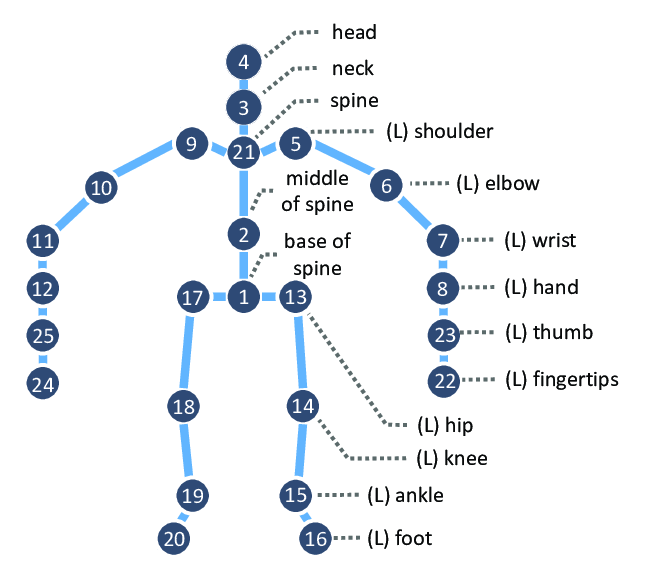
\includegraphics[width=.4\linewidth]{img/ntu_25joints.png}
	\caption{Illustration in \cite{9507447} showing the 25 joints of the human body based on NTU RGB+D.}\label{fig:ntu_25joints}
\end{figure}

\subsection{NTU RGB+D Dataset}
NTU RGB+D dataset proposed in 2016, was captured simultaneously using three Microsoft Kinect V2 sensors. It comprises 56,000 action sequences in 60 action classes, including 40 daily actions, 9 health-related actions, and 11 mutual actions. The data was collected from 40 volunteers, and each action sequence contains the three-dimensional positions of 25 body joints per frame, as shown in ~\ref{fig:ntu_25joints}. The dataset is divided into training and test sets using two different standards: Cross-Subject (X-Sub) and Cross-View (X-View). In the Cross-Subject setting, the dataset which contains 40320 samples and 16560 samples for training and evaluation, is split based on the person ID, resulting in 20 subsets for both the training and test sets. On the other hand, the Cross-View setting containing 37920 and 18960 samples for training and evaluation, divides the dataset according to camera ID. The samples collected by cameras 2 and 3 are used for training, while those collected by camera 1 are used for testing. Notably, the three cameras have horizontal angles differing by 45° each, ensuring diverse perspectives for robust evaluation.

\begin{figure}
	\centering
	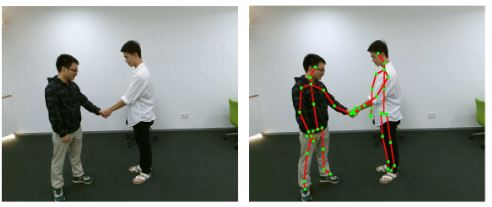
\includegraphics[width=.5\linewidth]{img/ntu_dataset.JPG}
	\caption{NTU RGB+D dataset \cite{Liu_2020} illustration of skeleton data.}\label{fig:ntu_dataset}
\end{figure}

\subsection{Drive\&Act Dataset}
The second dataset is the Drive\&Act dataset which is a significant benchmark for driver activity recognition, capturing activities in both manual and autonomous driving modes. This dataset offers a comprehensive collection of driver actions and interactions inside the vehicle cabin, providing valuable insights for driver monitoring and autonomous driving systems. The dataset consists of over 9.6 million frames, recorded from six different camera views and three modalities, collected by five Near-Infrared (NIR) and three RGB-D cameras. The data was recorded using a specially equipped vehicle that was driven on public roads in Germany. The vehicle was outfitted with six synchronized cameras placed in various positions. Three NIR cameras were utilized to capture images in low-light conditions, while three RGB-D cameras were used to capture color images and depth information. The synchronization ensured that all data streams were aligned in time, providing coherent multi-modal information for each frame. It includes skeleton data as one of its modalities. Specifically, the dataset includes 3D body and head pose data, which is represented as a time series of 3D rotation matrices. The skeleton data is captured using the OpenPose neural architecture, which is applied to each frame of the dataset that contains the driver's body or head.

The dataset comprises a hierarchical annotation scheme, offering rich semantic information about the driver's behavior. The annotations are organized into three levels:
\begin{itemize}
	\item \textbf{Coarse Tasks:} These represent high-level activities the drivers perform, such as "driving straight" or "turning left." These coarse tasks provide a broader context for understanding the driver's overall behavior.

	\item \textbf{Fine-Grained Activities:} These include more specific actions inside the vehicle cabin, such as "adjusting the radio" or "checking the rearview mirror." Fine-grained activities offer detailed insights into the driver's interactions and behaviors.

        \item \textbf{Atomic Action Units:} This level provides detailed triplets of annotations, including the driver's current action, the object they interact with, and the location of the object. This level of granularity allows for a deep analysis of the driver's actions and intentions.

\end{itemize}

The Drive\&Act dataset includes an extensive set of 83 fine-grained activity classes, surpassing previous driver activity recognition datasets by 62 additional activities. This broad range of actions enables a more comprehensive understanding of driver behavior. The dataset's size, with over 9.6 million frames, provides ample data for training and evaluation, making it one of the largest and most diverse datasets for driver activity recognition.

\begin{figure}
	\centering
	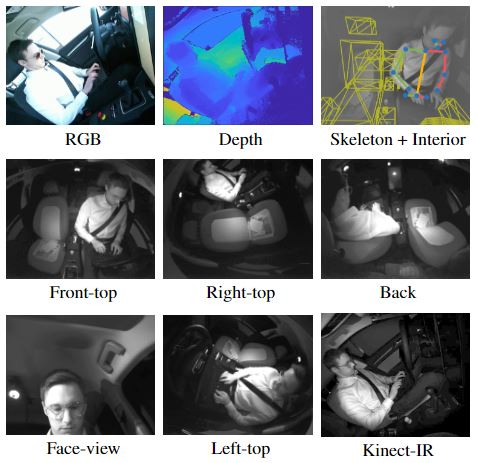
\includegraphics[width=.5\linewidth]{img/daa_dataset.JPG}
	\caption{Examples from Drive\&Act dataset \cite{drive_and_act_2019_iccv}, the "working on laptop" activity for different views and modalities.}\label{fig:ntu_dataset}
\end{figure}


\section{Data Preparation and Processing}
Preprocessing 3D skeleton data is a crucial step, considering its distinct nature compared to 2D images. In our experiments with both the NTU RGB+D and Drive\&Act datasets, we performed an in-depth analysis to gain a deeper understanding of the data and make informed decisions during preprocessing. Before diving into the preprocessing, a comprehensive visualization and analysis of the 3D skeleton data were performed. To gain a better understanding of the data, the 3D coordinates were projected onto 2 axes, allowing us to visualize the skeleton's movements and patterns, as shown in ~\ref{fig:ntu_visualisation}. This visualization helped in identifying any potential noise or inconsistencies in the data.

To improve model convergence and stability, data normalization was applied to both datasets. Normalization ensures that all 3D joint coordinates are within a consistent range, which is essential for the model's learning process. Specifically, each coordinate value was scaled to be between 0 and 1 by dividing it by the maximum value in the corresponding dimension across the entire dataset.

\begin{figure}
	\centering
	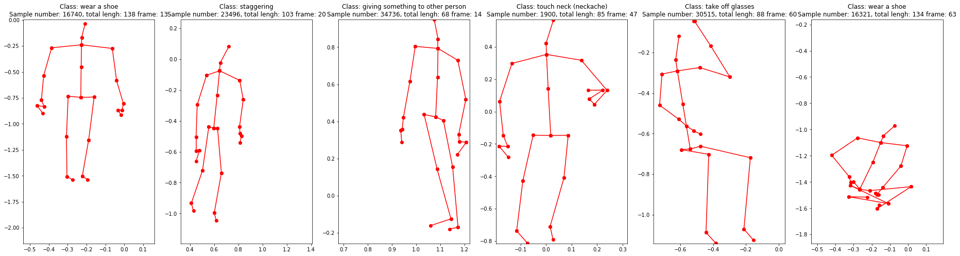
\includegraphics[width=\linewidth]{img/ntu_visualisation.png}
	\caption{Visualisations of the skeleton data from NTU RGB+D dataset plotted on x and y axes, showing the total frame of the sequence, the plotted frame, and the class label.}\label{fig:ntu_visualisation}
\end{figure}


Data augmentation is a fundamental aspect of contrastive learning, and it plays a crucial role in generating diverse views of the input skeleton sequences to enhance the model's ability to learn meaningful representations. In our preprocessing pipeline, we applied various spatial and temporal augmentations, including:

\begin{itemize}
	\item \textbf{Rotation:} An efficient spatial augmentation that randomly selected an axis (X, Y, or Z) as the main axis and applied a random rotation angle in the range [0, $\pi$/6] to it. The other two axes were also rotated with random angles in the range [0, $\pi$/180].
	\item \textbf{Crop:} As a temporal augmentation, Crop involved padding part of the frames in the original sequence and then randomly cropping it back to the original length. The padding ratio $\gamma$ was set to 1/6.
        \item \textbf{Spatial Flip:} Another spatial augmentation that swapped the left and right sides of the skeleton data with a probability of p=0.5, introducing additional variations in the data.
        \item \textbf{Shear:} A linear transformation was applied to the 3D coordinates using a shear matrix. The shear factors were randomly sampled from the range [-$\beta$, $\beta$], with $\beta$ set to 1 to control the augmentation strength.
 
\end{itemize}


\begin{figure}[htbp]
    \centering
    \subfigure{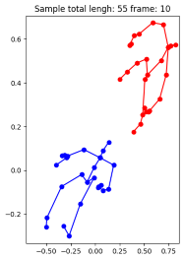
\includegraphics[width=0.3\textwidth]{img/ntu_rotation.png}}\hfill
    \subfigure{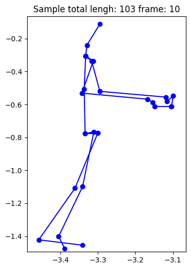
\includegraphics[width=0.3\textwidth]{img/ntu_visualisation1.png}}\hfill
    \subfigure{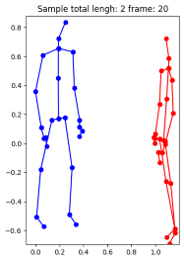
\includegraphics[width=0.3\textwidth]{img/ntu_visualisation2.png}}
    \caption{(a) Example of the rotation augmentation applied to the data. (b) Example shows a skeleton plot on the x and z axes. (c) Example shows samples with different subjects in the same frame.}
\end{figure}

These augmentations were applied to create different views of the skeleton sequences, enabling the model to capture diverse perspectives of the actions, leading to more robust and generalized representations. In addition to the ordinary augmentations described earlier, the second approach, PSTL, utilized specific masking strategies mentioned before in the Methodology chapter such as "Central Spatial Masking (CSM)" and "Motion Attention Temporal Masking (MATM)."

The data preprocessing and augmentation pipeline played a crucial role in preparing the NTU RGB+D and Drive\&Act datasets for training with the DINO and PSTL frameworks, respectively. Through visualization and analysis, normalization, and various data augmentations, we enhanced the datasets' quality and diversity, facilitating the models' ability to learn meaningful representations for effective human action recognition


The Drive\&Act dataset presented several challenges, especially when dealing with the skeleton modality. Unlike other modalities, such as RGB or NIR, only a few researchers have explored the skeleton data, making it an under-researched area. The skeleton data was extracted automatically from the N-IR modality using the OpenPose model for pose estimation. However, this led to a considerable number of errors in the annotation, including missing joints, shaded joints, and incorrect joint coordinates. Additionally, not all joints were consistently visible in the camera frame, particularly in the lower body region. Moreover, the actions in the Drive\&Act dataset exhibited similarity in terms of joint movements, making it challenging for the model to discriminate between action classes effectively. Furthermore, the dataset suffered from a significant class imbalance, with the class "sitting" being the most dominant among the 34 classes, as shown in ~\ref{fig:daa_dataset_class_visualization}.

\begin{figure}
	\centering
	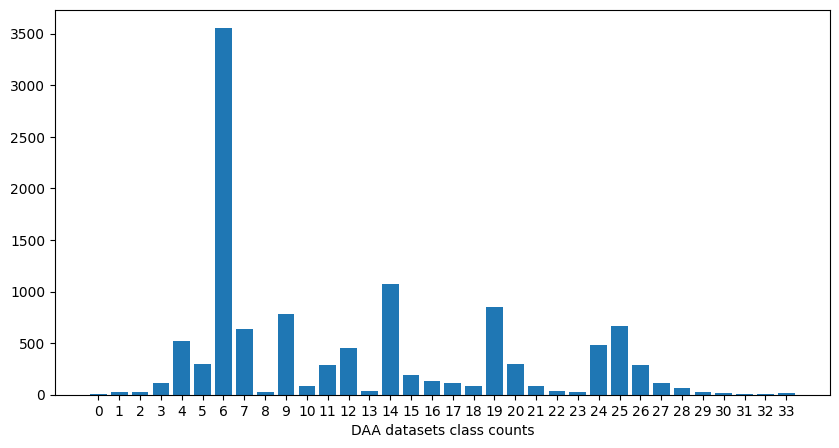
\includegraphics[width=.5\linewidth]{img/daa_dataset_class_visualization.png}
	\caption{Bar plot describing the class distribution of the Drive\&Act dataset.}\label{fig:daa_dataset_class_visualization}
\end{figure}

To address some of these issues, we decided to reduce the number of joints used in the model from 25 to 11, retaining only the most meaningful joints for better representation learning, as shown in ~\ref{fig:daa_visualization}. This will help the model focus on essential information and avoid redundancy in the data. Additionally, we employed the balanced accuracy metric during the evaluation phase to mitigate the impact of class imbalance, ensuring a fair assessment of the model's performance.

Despite the challenges and issues, the Drive\&Act dataset remains a valuable and challenging resource for driver activity recognition. Our comprehensive analysis and data preprocessing efforts aimed to create a meaningful and robust skeleton dataset, contributing to the exploration of self-supervised learning on this unique dataset. The findings from our experiments will shed light on the potential of using self-supervised learning for driver activity recognition and pave the way for future research in the Drive\&Act dataset.

\begin{figure}
	\centering
	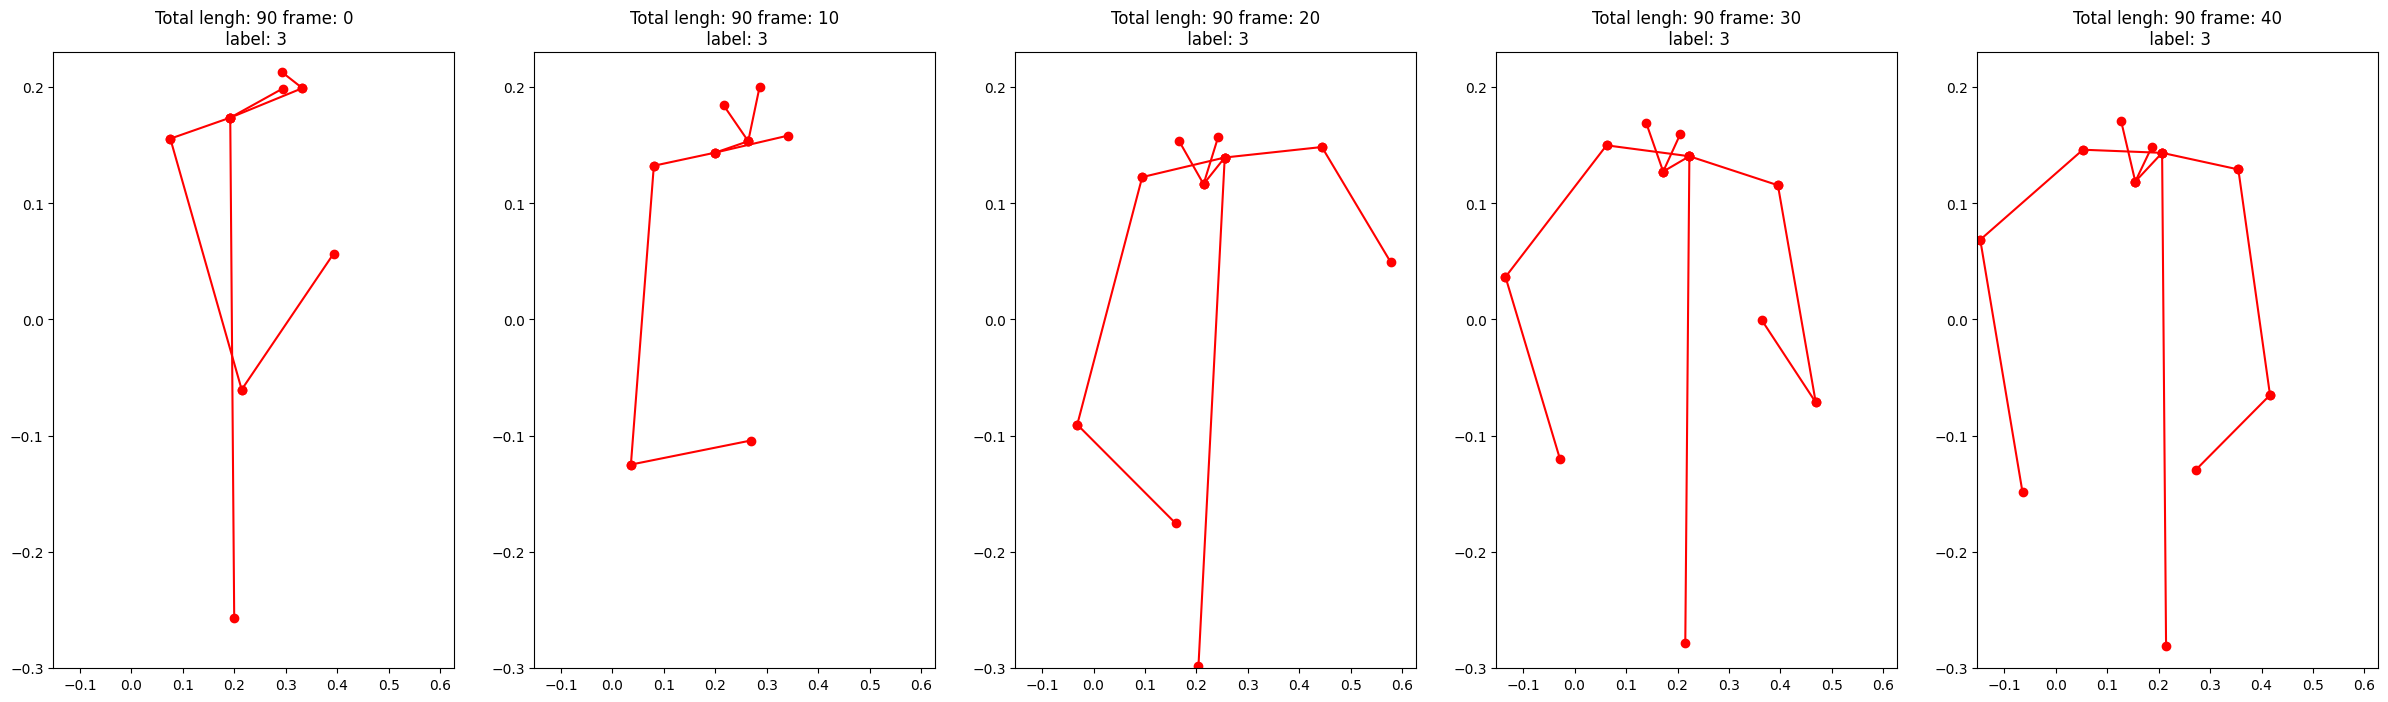
\includegraphics[width=.9\linewidth]{img/daa_sequence_visualization.png}
	\caption{Visualization of a skeleton sequence data from the Drive\&Act dataset with 11 joints. We can clearly see missing values in different frames.}\label{fig:daa_visualization}
\end{figure}

\section{Experiment Settings}
In our experimental settings, all experiments were conducted on a system equipped with 4 RTX A6000 GPUs. For the first approach, we used the NTU RGB+D dataset and the Drive\&Act dataset. To prepare the data for training, we padded the skeleton sequences to 120 frames for NTU RGB+D and 90 frames for Drive\&Act dataset. We employed the Stochastic Gradient Descent (SGD) optimizer with Nesterov momentum set to 0.9 and weight decay set to 0.0005. The loss function used was the cross entropy.

The training process for the first approach was performed over 90 epochs, with an initial learning rate of 0.3. To achieve better convergence, we used the CosineAnnealing scheduler for learning rate decay. The mini-batch size was set to 128 to balance computational efficiency and model performance. For the encoder architecture, we utilized STTFormer. In this approach, each tuple contained 6 consecutive frames, denoted as n=6. The STTFormer encoder comprised 8 spatio-temporal self-attention layers, with the output channels set to 64, 64, 128, 128, 256, 256, 256, and 256, respectively. The encoder network extracted 256-dimensional features from the skeleton sequences. To further refine the extracted features, two projectors were attached to the encoder network. Each projector consisted of 3 linear layers, with the first one followed by a batch normalization layer and leaky rectified linear units. The output size of the first linear layer was set to 512, while the final output dimension of the projector was 128.

A crucial aspect of the self-supervised learning approach is the temperature parameter, which determines the sharpness of the probability distribution. For the student network, we set the temperature parameter $\tau^s$ to 0.1, while for the teacher network, the temperature parameter $\tau^t$ was set to 0.03. This temperature scaling helped in fine-tuning the model's confidence during the contrastive learning process.

For the second approach, our experimental settings were tailored to the ST-GCN backbone and the specific requirements of PSTL. We resized the skeleton sequences to 50 frames for the NTU RGB+D dataset and 90 frames for the Drive\&Act dataset to create a suitable input length for the ST-GCN architecture.The ST-GCN backbone was configured with 16 hidden channels, which enabled the extraction of 256-dimensional features from the skeleton sequences. These features were further projected to 6144-dimensional embeddings to enhance the representation power of the model.

In the loss function of each stream, we set the value of $\lambda$ to 2e-4, which played a critical role in balancing the different components of the loss and guiding the learning process.To stabilize the training process, we utilized a 10-epoch warm-up phase, and the weight decay was set to 1e-5 to control overfitting and enhance the generalization ability of the model. During the pre-training and downstream tasks, we employed the Adam optimizer and the CosineAnnealing scheduler with 150 epochs. The mini-batch size was set to 128 for efficient computation.

For the evaluation of self-supervised learning, we utilized two protocols: linear evaluation and k-NN evaluation. In the linear evaluation, we added a linear classifier on top of the frozen pre-trained encoder and then trained the recognizer on the target skeleton action recognition dataset with an initial learning rate of 0.01. In the k-NN evaluation, we assessed the quality of features using a simple weighted k-Nearest Neighbor classifier. The pretrained model was frozen to compute and store the features of the training data for the downstream task. To classify a test skeleton $x$, we computed its representation and compared it against all stored training features, where k was set to 1. This evaluation protocol eliminated the need for hyperparameter tuning and data augmentation and could be run with only one pass over the downstream dataset, making it efficient and effective in evaluating the model's performance.


\chapter{Results}
In this section, we present the results of our experimental evaluations for both supervised and self-supervised learning approaches on the NTU RGB+D and Drive\&Act datasets. We start by analyzing the performance of the encoders ST-GCN and STTFormer in the supervised learning setting on the NTU RGB+D Dataset using both Cross-Subject (X-Sub) and Cross-View (X-View) evaluation protocols, as well as on the Drive\&Act dataset.

\section{Supervised Learning Results}

Table \ref{tab:supervised_results} summarizes the performance of the ST-GCN and STTFormer encoders in the supervised learning setting on the NTU RGB+D Dataset. The results are reported in terms of accuracy (\%) for both X-Sub and X-View evaluation protocols. We can observe that the STTFormer encoder achieves an accuracy of 84.3\% (X-Sub) and 94.3\% (X-View) on the NTU RGB+D dataset, outperforming the ST-GCN encoder, which achieves an accuracy of 81.5\% (X-Sub) and 88.3\% (X-View).

\begin{figure}
	\centering
	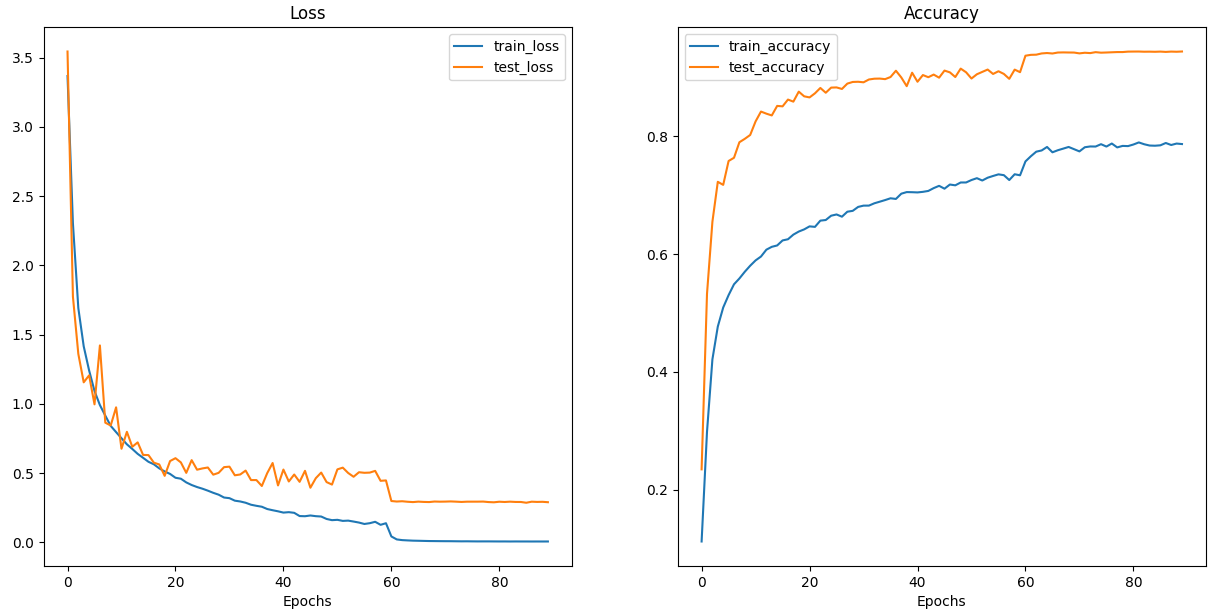
\includegraphics[width=.7\linewidth]{img/sttformer_loss_curves.png}
	\caption{STTFormer learning curve shows the loss function on the left and the accuracy metric on the right over the epochs.}\label{fig:sttformer_loss_curves}
\end{figure}


\begin{table}[htbp]
\centering
\caption{Supervised Learning Results on NTU RGB+D Dataset}
\label{tab:supervised_results}
\begin{tabular}{|c|c|c|}
\hline
\textbf{Encoder} & \textbf{NTU RGB+D (X-Sub)} & \textbf{NTU RGB+D (X-View)} \\
\hline
ST-GCN & 81.5\% & 88.3\% \\
\hline
STTFormer & 84.3\% & 94.3\% \\
\hline
\end{tabular}
\end{table}

The learning curve of the STTFormer is depicted in ~\ref{fig:sttformer_loss_curves}, illustrating the model's training progress in terms of both the loss function and accuracy. As training epochs increase, the loss function steadily decreases, indicating the model's improving ability to minimize the discrepancy between predicted and actual labels. Concurrently, the accuracy curve demonstrates a consistent upward trend, reflecting the STTFormer's increasing proficiency in correctly classifying action sequences. 

A visual representation of the model predictions on the NTU RGB+D dataset is depicted in ~\ref{fig:sttformer_predictions}, showcasing a 3 by 3 grid of action sequences. Each cell in the grid corresponds to a predicted action label, color-coded in red for false predictions and green for correct predictions. This illustrative example offers a snapshot of the model's performance in recognizing various human actions from the dataset.

The evaluation of the STTFormer and ST-GCN encoders on the Drive\&Act dataset yielded insightful results, shedding light on their performance in a car interior action recognition context. With a baseline accuracy of 2.9\% for random results, the challenge of accurate driver behavior recognition becomes evident, as mentioned before in the previous chapter regarding the challenges and issues of Drive\&Act dataset. The obtained accuracies of 5.03\% for the STTFormer and 9.05\% for the ST-GCN are indicative of their ability to capture subtle cues and patterns in driver actions within the vehicle cabin. \ref{tab:supervised_daa} presents a summary of the comparative performance of the two encoders on the Drive\&Act dataset, providing a clear overview of their respective accuracy outcomes.

\begin{figure}
	\centering
	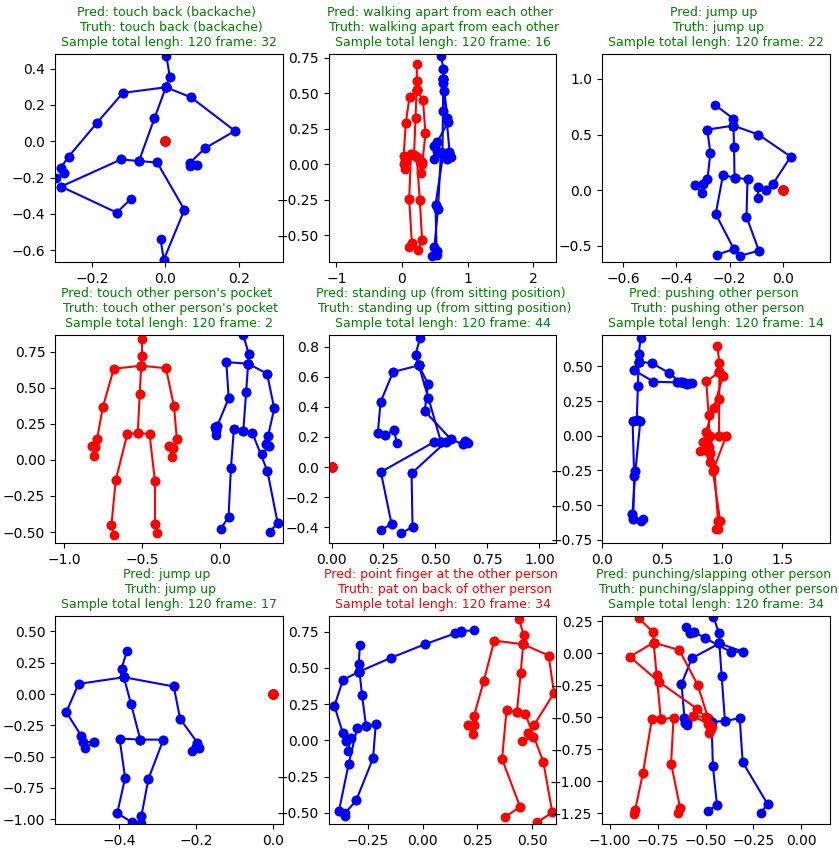
\includegraphics[width=.6\linewidth]{img/sttformer_predictions.png}
	\caption{Illustration showing STTFormer predictions on NTU RGB+D dataset.}\label{fig:sttformer_predictions}
\end{figure}

\begin{table}[h]
\centering
\begin{tabular}{|c|c|}
\hline
\textbf{Encoder} & \textbf{Accuracy} (\%) \\
\hline
Baseline & 2.9 \\
STTFormer & 5.03 \\
ST-GCN & 9.05 \\
\hline
\end{tabular}
\caption{Comparison of STTFormer and ST-GCN on Drive\&Act dataset}
\label{tab:supervised_daa}
\end{table}

The outcomes obtained from the supervised learning evaluation provide valuable insights into the potential performance of the subsequent self-supervised learning approach. By establishing a baseline of accuracy using traditional supervised methods, we gain a clearer understanding of the inherent challenges and intricacies of the action recognition task. This baseline performance serves as a benchmark against which the SSL approach can be measured, enabling us to gauge the extent to which self-supervised learning enhances recognition capabilities. The supervised learning results thus lay the foundation for assessing the efficacy and contributions of SSL in capturing meaningful representations from unannotated skeleton data, ultimately informing our expectations and interpretations of the subsequent SSL results.

\section{Self-Supervised Learning Results}
The self-supervised learning results for the two approaches, PSTL \& ST-GCN and DINO \& STTFormer, on the NTU RGB+D dataset are presented in the table \ref{tab:ssl_knn_ntu}, and result of SSL for the two approaches on the Drive\&Act dataset, presented in \ref{tab:ssl_knn_daa}:

\begin{table}[h]
\centering
\caption{SSL Results on NTU RGB+D Dataset with k-NN evaluation}
\label{tab:ssl_knn_ntu}
\begin{tabular}{|l|c|c|}
\hline
Approach & Evaluation Type & Accuracy (\%) \\
\hline
DINO \& STTFormer & k-NN (X-sub) & 23.02 \\
DINO \& STTFormer & k-NN (X-view) & 30.04 \\
\hline
PSTL \& ST-GCN & k-NN (X-sub) & 58.65 \\
PSTL \& ST-GCN & k-NN (X-view) & 66.06 \\
\hline
\end{tabular}
\end{table}


\begin{table}[h]
\centering
\caption{SSL Results on Drive\&Act Dataset}
\label{tab:ssl_knn_daa}
\begin{tabular}{|c|c|}
\hline
Approach & k-NN Evaluation Accuracy (\%) \\
\hline
DINO \& STTFormer & 2.94 \\
PSTL \& ST-GCN & 5.37 \\
\hline
\end{tabular}
\end{table}


The second approach outperformed the first in terms of k-NN evaluation accuracy on the NTU RGB+D dataset. This difference in performance could be attributed to several factors. The PSTL strategy introduced in the second approach, which involves partial spatio-temporal learning and masking strategies, likely contributed to capturing more discriminative and relevant information from the skeleton sequences. The utilization of the ST-GCN architecture as the backbone may have enabled better feature extraction from the skeleton data, leading to improved action recognition. Also, The observed difference in performance between the STTFormer and ST-GCN approaches could be influenced by the nature of transformer-based models like STTFormer, which typically require larger amounts of data in the DINO context to reach their full potential. In contrast, the ST-GCN model, being a graph convolutional network, might exhibit relatively better performance with smaller datasets. This characteristic could have contributed to the superior performance of the ST-GCN approach, as the NTU RGB+D dataset, though sizable, may not fully satiate the data hunger of the STTFormer architecture. The interplay between model architecture and dataset size underscores the importance of matching the learning capacity of the model with the available data, potentially explaining part of the observed performance disparity. Furthermore, the PSTL strategy's focus on leveraging the human skeleton graph's topological structure and motion patterns might have enhanced the model's ability to learn meaningful representations. In contrast, while the DINO \& STTFormer approach harnessed the self-distillation technique and the STTFormer as the encoder, its performance might have been influenced by challenges such as convergence during training and limited capability to generalize across domains. These results collectively indicate that the PSTL \& ST-GCN approach's design and features potentially align well with the specific characteristics of human action recognition tasks, contributing to its superior performance compared to the DINO \& STTFormer approach.


The second approach, employing the PSTL \& ST-GCN framework, was further evaluated on both the NTU RGB+D and Drive\&Act datasets, showcasing its adaptability and performance in various contexts, as shown in \ref{tab:pstl_experiments}. The linear evaluation on the NTU RGB+D dataset yielded promising results, with accuracy values of 76.76\% (X-Sub) and 82.56\% (X-View), demonstrating the effectiveness of the approach in learning meaningful representations. Finetuning the model on this dataset further improved the performance, achieving accuracies of 84.2\% (X-Sub) and 91.6\% (X-View) which is better by +2.7\% and +3.3\% respectively compared to training the model from scratch, validating the capacity of the learned features for downstream tasks. Additionally, the linear evaluation on the Drive\&Act dataset yielded an accuracy of 14.6\%, indicating the potential of the model for recognizing driver actions within the car interior.

Cross-evaluation between datasets involves training a model on one dataset and evaluating it on a different, distinct dataset. This process assesses the model's ability to generalize its learned representations across domains and adapt to new and unseen data. In the context of action recognition, cross-evaluation helps validate the robustness and transferability of the learned features, enabling the model to recognize actions in diverse environments or scenarios. Notably, the cross-evaluation between the two datasets revealed an accuracy of 3.91\%, where it was pretrained on NTU RGB+D and evaluated on Drive\&Act.

\begin{table}[h]
\centering
\caption{Results of PSTL \& ST-GCN Approach}
\label{tab:pstl_experiments}
\begin{tabular}{|c|c|c|}
\hline
Dataset & Evaluation Type & Accuracy (\%) \\
\hline
NTU RGB+D & Linear Evaluation (X-Sub) & 76.76 \\
NTU RGB+D & Linear Evaluation (X-View) & 82.56 \\
NTU RGB+D & Finetune (X-Sub) & 84.2 \\
NTU RGB+D & Finetune (X-View) & 91.6 \\
Drive\&Act & Linear Evaluation & 14.6 \\
Cross-Evaluation & NTU RGB+D to Drive\&Act & 3.91 \\
\hline
\end{tabular}
\end{table}



\section{Ablation Studies on Drive\&Act Dataset}
In pursuit of optimizing the performance of the Drive\&Act dataset, several experiments were conducted, each aiming to uncover insights into the dataset's characteristics. The first set of experiments focused on varying the number of joints used for action recognition, as shown in \ref{tab:daa_experiment1}. Interestingly, while reducing the number of joints to 11 initially seemed like a strategy to improve performance by filtering out potentially irrelevant data, the results demonstrated that further reduction below this threshold led to a decline in accuracy. This suggests that even seemingly minor joints contribute valuable information for accurate action recognition within the car environment. 

\begin{table}[h]
\centering
\caption{Joint Variation Experiment:}
\label{tab:daa_experiment1}
\begin{tabular}{|c|c|c|}
\hline
\textbf{Dataset} & \textbf{Number of Joints} & \textbf{k-NN Evaluation Accuracy} \\
\hline
Drive\&Act & 11 joints & 5.37\% \\
\hline
Drive\&Act & 8 joints & 4.3\% \\
\hline
\end{tabular}
\end{table}

In the second set of experiments, the number of frames in the skeleton sequences was adjusted. Analyzing the dynamics of the Drive\&Act dataset revealed that a significant portion of action-related movements occurred within the final frames of the sequences, as shown in \ref{tab:daa_experiment2}. This is in contrast to the NTU RGB+D dataset, where actions predominantly occur in the first 50 frames. The experiments validated this observation, as reducing the sequence length to 50 frames led to a dip in performance. This finding underscores the importance of capturing the complete temporal context of actions within the car cabin, highlighting the distinct characteristics of the Drive\&Act dataset compared to other datasets. 

\begin{table}[h]
\centering
\caption{Sequence Length Experiment:}
\label{tab:daa_experiment2}
\begin{tabular}{|c|c|c|}
\hline
\textbf{Dataset} & \textbf{Number of Frames} & \textbf{k-NN Evaluation Accuracy} \\
\hline
Drive\&Act & 90 frames & 5.37\% \\
\hline
Drive\&Act & 50 frames & 3.98\% \\
\hline
\end{tabular}
\end{table}

The results of these experiments emphasize the intricacies of the Drive\&Act dataset and shed light on the interplay between the number of joints and sequence length for effective action recognition. This understanding is crucial for fine-tuning model architectures and training strategies.

\section{Comparison with the State-of-the-Art Methods}
In the realm of human action recognition, comparing self-supervised learning approaches with state-of-the-art methods provides valuable insights into the advancements made in this field. In \ref{tab:state_of_the_art}, we present the results of the linear evaluation on the NTU RGB+D dataset. The second approach PSTL \cite{zhou2023self} with ST-GCN, in our implementation, achieves competitive performance, yielding 76.76\% accuracy on the xsub evaluation and 82.56\% accuracy on the xview evaluation. This places the method among the top performers in terms of accuracy, showcasing the efficacy of self-supervised learning for skeleton-based action recognition. Notably, the PSTL with ST-GCN approach demonstrates a notable leap in accuracy over existing methods, such as AimCLR, which achieved 74.3\% and 79.7\% accuracy on the xsub and xview evaluations, respectively. These results underscore the potential of self-supervised learning, particularly the PSTL framework, in enhancing state-of-the-art performance in human action recognition. 

\begin{table}[h]
\centering
\caption{Linear evaluation results of state-of-the-art on NTU RGB+D dataset. \textbf{*} indicates our implementation of the approach.}
\label{tab:state_of_the_art}
\begin{tabular}{|l|cc|}
\hline Method & \multicolumn{2}{|c|}{NTU-60 (\%)} \\
& xsub & xview \\
\hline
MS2L (ACM MM 20) \cite{lin2020ms2l} & 52.6 & - \\
P\&C (CVPR 20) \cite{su2020predict} & 50.7 & 76.3 \\
AS-CAL (Inf Sci 21) \cite{rao2021augmented} & 58.5 & 64.8 \\
AimCLR (AAAI 22) \cite{guo2022contrastive} & 74.3 & 79.7 \\
PSTL \& ST-GCN & 77.3 & 81.8 \\
PSTL \& ST-GCN \textbf{*} & 76.8 & 82.6 \\
\hline
\end{tabular}
\end{table}

\section{Discussion}
The results obtained through extensive evaluations shed light on various aspects of the proposed self-supervised learning approaches for action recognition using 3D skeleton data. Notably, the comparison of the two approaches, DINO with STTFormer and PSTL with ST-GCN, underscores the potential benefits of self-supervised learning over traditional supervised learning paradigms. Self-supervised learning offers a pathway to harnessing unannotated data for representation learning, enhancing model performance in downstream tasks.

It is intriguing to observe that while k-NN evaluation often yields lower accuracy compared to Linear evaluation, k-NN evaluation possesses its own distinct advantages. The lower accuracy of k-NN evaluation can be attributed to the method's inherent simplicity and reliance on a smaller number of parameters, which might limit its adaptability to various scenarios. However, k-NN evaluation provides an insightful mechanism for probing the quality of learned representations. The nearest-neighbor approach tests the model's ability to map similar actions to neighboring points in the feature space, making it a valuable tool for assessing the model's capability to cluster semantically related actions.

In the context of supervised learning, the linear evaluation of the PSTL \& ST-GCN approach demonstrates substantial improvement over traditional ST-GCN on the NTU RGB+D dataset. The model's adaptability to different domains is exemplified by cross-evaluation, where the model pretrained on NTU RGB+D showcased a 3.91\% accuracy when evaluated on the distinct Drive\&Act dataset. This cross-evaluation can demonstrate the potential of the learned features if they can generalize across datasets and environments, a key aspect in ensuring the model's robustness.

Furthermore, insights into the unique characteristics of the Drive\&Act dataset were garnered through targeted experiments. Varying the number of joints for action recognition illustrated that, contrary to initial assumptions, reducing the number of joints below 11 resulted in decreased accuracy. This emphasizes the importance of even seemingly minor joints in capturing essential information for accurate action recognition within the car environment. Additionally, the impact of sequence length on model performance was revealed, showcasing the necessity of capturing complete temporal contexts in the Drive\&Act dataset, which is distinct from other datasets like NTU RGB+D.

Collectively, these discussions highlight the intricate interplay between self-supervised learning, evaluation methodologies, model architecture, and dataset characteristics. The findings underscore the potential of self-supervised learning for advancing action recognition in diverse environments and lay the groundwork for future research endeavors in this promising domain.

In this section, we presented comprehensive results stemming from our exploration of self-supervised learning for human action recognition using 3D skeleton representations. We began by evaluating the performance of two encoders, ST-GCN and STTFormer, through supervised learning on the NTU RGB+D and Drive\&Act datasets. These supervised learning results provided valuable insights into the capabilities of the encoders and laid the foundation for our subsequent self-supervised learning experiments. We then delved into our self-supervised approach, DINO with STTFormer, and second approach PSTL with ST-GCN, showcasing their performance on both benchmark datasets. Through meticulous analysis, we observed that the PSTL with ST-GCN approach exhibited promising results, especially on the NTU RGB+D dataset, rivaling state-of-the-art methods. Our exploration of various parameters and techniques, including data augmentation and model architecture, contributed to a deeper understanding of the potential of self-supervised learning for enhancing action recognition systems. The promising outcomes underscore the significance of self-supervised learning in advancing the field of human action recognition and lay the groundwork for future research and applications.
\chapter{Conclusion}
This master thesis was motivated by the increasing concern over the rising number of car accidents caused by driver distraction and the need for advanced action recognition systems to promote road safety. The main purpose of this thesis was to enhance vehicle interior action recognition using self-supervised learning with 3D human skeleton representations. By utilizing unannotated data, self-supervised learning offers a promising approach to learning meaningful representations for action recognition without the need for labor-intensive annotations.

To achieve our research objectives, we investigated two different approaches for SSL: DINO with STTFormer and PSTL with ST-GCN. The second approach showed promising results in extracting meaningful features from 3D human skeleton representations and demonstrated the potential of self-supervised learning for action recognition in the car interior. Throughout our investigation, we carefully selected evaluation protocols and conducted comprehensive comparisons to answer our research question about recognizing human action based on skeleton data using self-supervised learning. Our experimental results showed that PSTL with ST-GCN achieved competitive performance in action recognition on the NTU RGB+D and the approach DINO with STTFormer has its limitations and needs further research. 

The application of DINO with STTFormer to the task of skeleton-based action recognition encountered certain limitations that hindered its performance. One possible reason for its suboptimal results lies in the fact that the DINO framework has primarily showcased strong performance on image data, which inherently contains a vast amount of information due to the sheer number of pixels. In contrast, skeleton data represents a compressed form of human action, encapsulating movement patterns with fewer dimensions. This limitation also extends to STTFormer, a variant of Transformers that may require a larger volume of data to achieve optimal performance. Additionally, the DINO framework was initially designed for static images, while our task involves sequential data in the form of skeleton sequences. These factors collectively suggest that DINO's efficacy may be hampered when applied directly to skeleton-based action recognition. To further validate the potential of DINO, future research could explore alternative encoders, such as ST-GCN, within the DINO framework. This investigation would provide a more comprehensive understanding of DINO's adaptability and effectiveness for our specific task.

During our exploration of the Drive\&Act dataset, we encountered several challenges, including errors in annotating the dataset, issues with missing or incorrect joint coordinates, and the presence of highly imbalanced classes. To overcome these challenges and achieve better results, future work is needed to develop improved techniques for dealing with the skeleton modality in the Drive\&Act dataset. Additionally, there is an urgent need to create more high-quality datasets dedicated to human action recognition inside the car, which will facilitate the development and evaluation of more accurate and robust action recognition systems.

Furthermore, an area of future research lies in improving the interpretability of self-supervised learning models. As these models learn representations in a self-supervised manner, understanding the learned features and how they correspond to specific human actions and behaviors remains a valuable avenue for exploration.

Throughout the course of this master's thesis, I have delved into the realm of contrastive self-supervised learning for action recognition using 3D skeleton data, a topic that continues to be at the forefront of research and exploration. This endeavor has illuminated the promising potential of applying such techniques to diverse domains, including the recognition of human actions. As I delved into the intricacies of analyzing and evaluating skeleton data, I gained valuable insights into the nuances of this unique data type, which diverges from the more commonly encountered image data. Moreover, this thesis provided an invaluable opportunity to learn how to construct intricate models and architectures, harnessing the power of parallel GPUs to accelerate training processes on server setups.

The journey through this research venture has been a master class in evaluation methodologies. The mastery of diverse evaluation techniques, ranging from k-NN and Linear evaluation to finetuning and cross-evaluation, was particularly enlightening. Each of these approaches granted me a multifaceted perspective on the performance of the proposed methods, enabling comprehensive insights into their strengths and limitations.Another pivotal aspect of this master's thesis was the experience of dealing with various datasets, each accompanied by its distinct set of challenges. This hands-on experience underscored the importance of data preprocessing and augmentation, as well as the need to carefully design experiments to achieve meaningful and reliable results. 


In conclusion, this master thesis has provided valuable insights into the potential of self-supervised learning for human action recognition in the car interior. By leveraging 3D human skeleton representations and employing contrastive learning techniques, our study contributes to the advancement of action recognition systems for improving road safety and driver assistance in both manual and autonomous driving scenarios. The future of self-supervised learning in this domain looks promising, and continued research in this field is vital to unlocking the full potential of action recognition systems for enhanced vehicle safety.

%\input{ChapterExample}

\bibliographystyle{IEEEtran}
\bibliography{references}
\end{document}
